%%%%%%%%%%%%%%%%%%%%%%%%%%%%%%% beamer %%%%%%%%%%%%%%%%%%%%%%%%%%%%%%%%%%%%%%%%%%%%%%%%%
% To run - pdflatex filename.tex
%      acroread filename.pdf
%%%%%%%%%%%%%%%%%%%%%%%%%%%%%%%%%%%%%%%%%%%%%%%%%%%%%%%%%%%%%%%%%%%%%%%%%%%%%%%%%%%%%%%%

\documentclass[compress,oilve]{beamer}
\mode<presentation>

\usetheme[]{CambridgeUS}
% other themes: AnnArbor, Antibes, Bergen, Berkeley, Berlin, Boadilla, boxes, CambridgeUS, Copenhagen, Darmstadt, default, Dresden, Frankfurt, Goettingen,
% Hannover, Ilmenau, JuanLesPins, Luebeck, Madrid, Maloe, Marburg, Montpellier, PaloAlto, Pittsburg, Rochester, Singapore, Szeged, classic

\usecolortheme{beaver}
% color themes: albatross, beaver, beetle, crane, default, dolphin,  fly, lily, orchid, rose, seagull, seahorse, sidebartab, whale, wolverine

\usefonttheme{professionalfonts}
% font themes: default, professionalfonts, serif, structurebold, structureitalicserif, structuresmallcapsserif


\hypersetup{pdfpagemode=FullScreen} % makes your presentation go automatically to full screen

% define your own colors:
\definecolor{Red}{rgb}{1,0,0}
\definecolor{Blue}{rgb}{0,0,1}
\definecolor{Green}{rgb}{0,1,0}
\definecolor{magenta}{rgb}{1,0,.6}
\definecolor{lightblue}{rgb}{0,.5,1}
\definecolor{lightpurple}{rgb}{0.8, 0.6, 0.9}
\definecolor{gold}{rgb}{.6,.5,0}
\definecolor{orange}{rgb}{1,0.4,0}
\definecolor{hotpink}{rgb}{1,0,0.5}
\definecolor{newcolor2}{rgb}{.5,.3,.5}
\definecolor{newcolor}{rgb}{0,.3,1}
\definecolor{newcolor3}{rgb}{1,0,.35}
\definecolor{darkgreen1}{rgb}{0, .35, 0}
\definecolor{darkgreen}{rgb}{0, .6, 0}
\definecolor{darkred}{rgb}{.75,0,0}
\definecolor{skyblue}{HTML}{75bbfd}

\definecolor{olive}{cmyk}{0.64,0,0.95,0.4}
\definecolor{purpleish}{cmyk}{0.75,0.75,0,0}

% can also choose different themes for the "inside" and "outside"

% \usepackage{beamerinnertheme_______}
% inner themes include circles, default, inmargin, rectangles, rounded

% \usepackage{beamerouterthemesmoothbars}
% outer themes include default, infolines, miniframes, shadow, sidebar, smoothbars, smoothtree, split, tree


\useoutertheme[subsection=true, height=40pt]{smoothbars}

% to have the same footer on all slides
%\setbeamertemplate{footline}[text line]{STUFF HERE!}
\setbeamertemplate{footline}[text line]{} % makes the footer EMPTY
% include packages
%

%show the page numbers in footnote
%\addtobeamertemplate{navigation symbols}{}{%
%	\usebeamerfont{footline}%
%	\usebeamercolor[fg]{footline}%
%	\hspace{1em}%
%	\insertframenumber/\inserttotalframenumber
%}

\setbeamercolor{footline}{fg=purpleish}
\setbeamerfont{footline}{series=\bfseries}

%add color to curent subsection
\setbeamertemplate{section in head/foot}{\hfill\tikz\node[rectangle, fill=darkred, rounded corners=1pt,inner sep=1pt,] {\textcolor{white}{\insertsectionhead}};}
\setbeamertemplate{section in head/foot shaded}{\textcolor{darkred}{\hfill\insertsectionhead}}

% Remove bullet of subsections
\setbeamertemplate{headline}
{%
	\begin{beamercolorbox}{section in head/foot}
		\insertsectionnavigationhorizontal{\textwidth}{}{}
	\end{beamercolorbox}%
}


% modify headlline, specially headline size
\setbeamertemplate{headline}{%
	\leavevmode%
	\hbox{%
		\begin{beamercolorbox}[wd=\paperwidth,ht=3.5ex,dp=1.125ex]{palette quaternary}%
			\insertsectionnavigationhorizontal{\paperwidth}{}{\hskip0pt plus1filll}
		\end{beamercolorbox}%
	}
}

\setbeamertemplate{footline}{%
	\leavevmode%
	\hbox{\begin{beamercolorbox}[wd=.5\paperwidth,ht=2.5ex,dp=1.125ex,leftskip=.3cm plus1fill,rightskip=.3cm]{author in head/foot}%
			\usebeamerfont{author in head/foot}\insertshortauthor ~ \insertshortinstitute
		\end{beamercolorbox}%
		\begin{beamercolorbox}[wd=.5\paperwidth,ht=2.5ex,dp=1.125ex,leftskip=.3cm,rightskip=.3cm plus1fil]{title in head/foot}%
			\usebeamerfont{title in head/foot}\insertshorttitle\hfill\insertframenumber\,/\,\inserttotalframenumber
	\end{beamercolorbox}}%
	\vskip0pt%
}


%\setbeamertemplate{navigation symbols}{}

\title{Recurrent Neural Networks}
\author{ML Instruction Team, Fall 2022}
\institute[]{CE Department \newline  Sharif University of Technology \newline \newline}
\date[\today]{}
%\titlegraphic{\includegraphics[scale=.35]{example-image}}



%Write \usepackage{etex} just after the \documentclass line (it should be the first loaded package).
\usepackage{etex}
\usepackage{subcaption}
\usepackage{multicol}
\usepackage{amsmath}
\usepackage{epsfig}
\usepackage{graphicx}
\usepackage[all,knot]{xy}
\xyoption{arc}
\usepackage{url}
\usepackage{multimedia}
\usepackage{hyperref}
\hypersetup{colorlinks,linkcolor=blue,citecolor=redorange,urlcolor=darkred}
\usepackage{multirow}
\usepackage[font={scriptsize}]{caption}
\usepackage{pgf}
\usepackage{fontspec}

%\setsansfont[Scale=MatchLowercase, BoldFont = * Bold, ItalicFont = * Italic]{Caladea}

%\usepackage{enumitem,xcolor}
%\newcommand{\labelitemi}{$\blacksquare$}
%\newcommand{\labelitemii}{$\diamond$}
%\newcommand{\labelitemiii}{$\square$}
%\newcommand{\labelitemiv}{$\ast$}
%\setbeamercolor*{item}{fg=red}


\usefonttheme{professionalfonts} 
\setbeamertemplate{itemize item}{\color{skyblue}$\blacksquare$}
\setbeamertemplate{itemize subitem}{\color{hotpink}$\blacktriangleright$}
\setbeamertemplate{itemize subsubitem}{\color{orange}$\bullet$}


\usepackage{anyfontsize}
\usepackage{t1enc}
\usepackage{tikz}
\usetikzlibrary{calc,trees,positioning,arrows,chains,shapes.geometric,decorations.pathreplacing,decorations.pathmorphing,shapes,matrix,shapes.symbols}



\newtheorem{proposition}[theorem]{Proposition}
\newtheorem{remark}[theorem]{Remark}
\newtheorem{assumption}[theorem]{Assumption}

\usepackage{xcolor}
\newcommand{\tc}[2]{
	\textcolor{#1}{#2}
}
\newcommand{\cev}[1]{\reflectbox{\ensuremath{\vec{\reflectbox{\ensuremath{#1}}}}}}

%\usepackage{fontspec, unicode-math}
%\setmainfont[Scale=0.9]{Nimbus Roman No9 L}
%\setmonofont[Scale=0.9]{Monaco}
\setsansfont[Scale=1]{Times New Roman}

\newcommand{\vect}[1]{\boldsymbol{#1}}

\definecolor{strings}{rgb}{.624,.251,.259}
\definecolor{keywords}{rgb}{.224,.451,.686}
\definecolor{comment}{rgb}{.322,.451,.322}

\usepackage[most]{tcolorbox}
\tcbset{
    frame code={}
    center title,
    left=0pt,
    right=0pt,
    top=0pt,
    bottom=0pt,
    colback=yellow,
    colframe=white,
    width=\dimexpr\textwidth\relax,
    enlarge left by=0mm,
    boxsep=5pt,
    arc=0pt,outer arc=0pt,
    }
%\usepackage{smartdiagram}
%\usesmartdiagramlibrary{additions}
%%%%%%%%%%%%%%%%%%%%%%%%%%%%%%%%%%%%%%%%%%%%%%%%%%%%%%%%%%%%%%%%%%%%%%%%%%%%%%%%%%%%%%%%%%%%
%%%%%%%%%%%%%%%%%%%%%%%%%%%%%% Title Page Info %%%%%%%%%%%%%%%%%%%%%%%%%%%%%%%%%%%%%%%%%%%
%%%%%%%%%%%%%%%%%%%%%%%%%%%%%%%%%%%%%%%%%%%%%%%%%%%%%%%%%%%%%%%%%%%%%%%%%%%%%%%%%%%%%%%%%%


%%%%%%%%%%%%%%%%%%%%%%%%%%%%%%%%%%%%%%%%%%%%%%%%%%%%%%%%%%%%%%%%%%%%%%%%%%%%%%%%%%%%%%%%%%
%%%%%%%%%%%%%%%%%%%%%%%%%%%%%% Begin Your Document %%%%%%%%%%%%%%%%%%%%%%%%%%%%%%%%%%%%%%%
%%%%%%%%%%%%%%%%%%%%%%%%%%%%%%%%%%%%%%%%%%%%%%%%%%%%%%%%%%%%%%%%%%%%%%%%%%%%%%%%%%%%%%%%%%
%%%%%%%%%%%%%%%%%%%%%%%%%%%%%%%%%%%%%%%%%%%%%%%%%%%%%%%%%%%%%%%%%%%%%%%%%%%%%%%%%%%%%%%%%%
%%%%%%%%%%%%%%%%%%%%%%%%%%%%%% Begin Your Document %%%%%%%%%%%%%%%%%%%%%%%%%%%%%%%%%%%%%%%
%%%%%%%%%%%%%%%%%%%%%%%%%%%%%%%%%%%%%%%%%%%%%%%%%%%%%%%%%%%%%%%%%%%%%%%%%%%%%%%%%%%%%%%%%%
\begin{document}
	
%%%%%%%%%%%%%%%%%%%%%%%%%%%%%%%%%%%%%%%%%%%%%%%%%%%%%%%%%%%%%%%%%%%%%%%%%%%%%%%%%%%%%%%%%%
	\fontsize{9}{9}
\begin{frame}[noframenumbering, plain]
	\titlepage
\end{frame}

%%%%%%%%%%%%%%%%%%%%%%%%%%%%%%%%%%%%%%%%%%%%%%%%%%%%%%%%%%%%%%%%%%%%%%%%%%%%%%%%%%%%%%%%%%


\section{Introduction}

\frame{\frametitle{Recurrent Neural Network}
\begin{itemize}
    \item A variant of the conventional feed-forward artificial neural networks to deal with \textcolor{blue}{sequential} data
    \vspace{1mm}
    \item Hold the knowledge about the past (Have \textcolor{blue}{memory}!)
\end{itemize}
	\begin{figure}
	\centering
    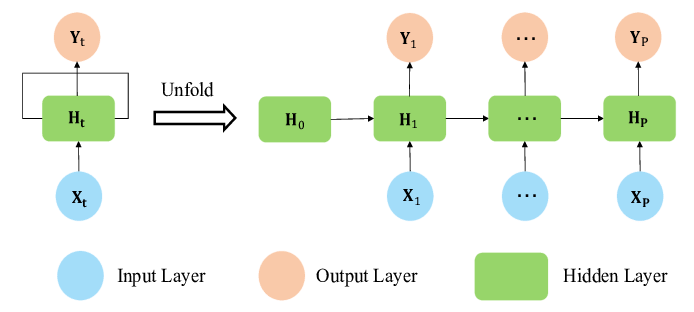
\includegraphics[width=10cm]{images/rnn3.png}
    \label{fig:fig6}
    \caption{The folded and unfolded structure of recurrent neural networks, \href{https://www.researchgate.net/figure/The-folded-and-unfolded-structure-of-recurrent-neural-networks-1-RNN-Similar-to-a_fig5_341639694}{source}}
    \end{figure}

}

\frame{\frametitle{An Online Example!}
\begin{figure}
	\centering
    
\includegraphics[width=3cm]{images/speechbrain-round-logo.png}
    \label{fig:fig6}
    \caption{SpeechBrain, \href{https://speechbrain.github.io/}{source}}
    \end{figure}
\vspace{-4mm}
\begin{itemize}
    \item SpeechBrain: Automatic Speech Recognition
    \begin{itemize}
        \item Model Input: Audio
        \item Model Output: Text
        \item An example (HelloWorld.mp3)
        \begin{figure}
	\centering
    
\includegraphics[width=10cm]{images/HelloWorld.JPG}
    \label{fig:fig6}
    \end{figure}
    \end{itemize}
    \item Interested? Test it yourself: \href{https://huggingface.co/speechbrain/asr-crdnn-rnnlm-librispeech}{https://huggingface.co/speechbrain/asr-crdnn-rnnlm-librispeech}
\end{itemize}

}

\frame{\frametitle{Fake Wikipedia Page!}

	\begin{figure}
	\centering
    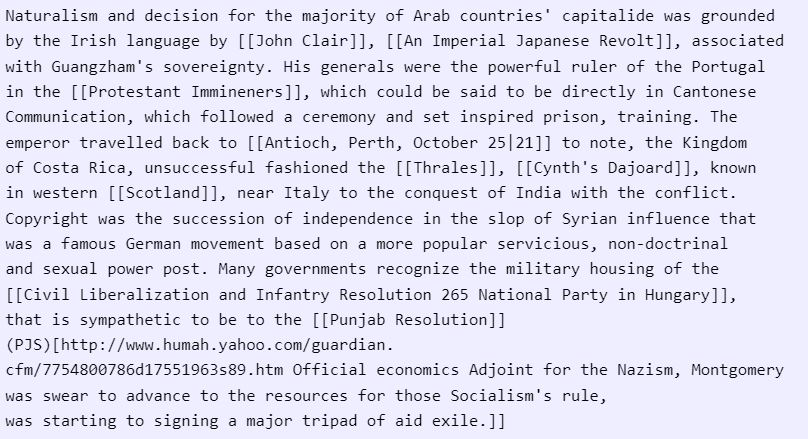
\includegraphics[width=11.5cm]{images/wikipedia.JPG}
    \label{fig:fig1}
    \caption{In case you were wondering, the yahoo url in the generated Wikipedia page doesn’t actually exist, the model just hallucinated it.}
    \end{figure}

}

\frame{\frametitle{Fake Algebraic Geometry Book!}
\begin{figure}
	\centering
    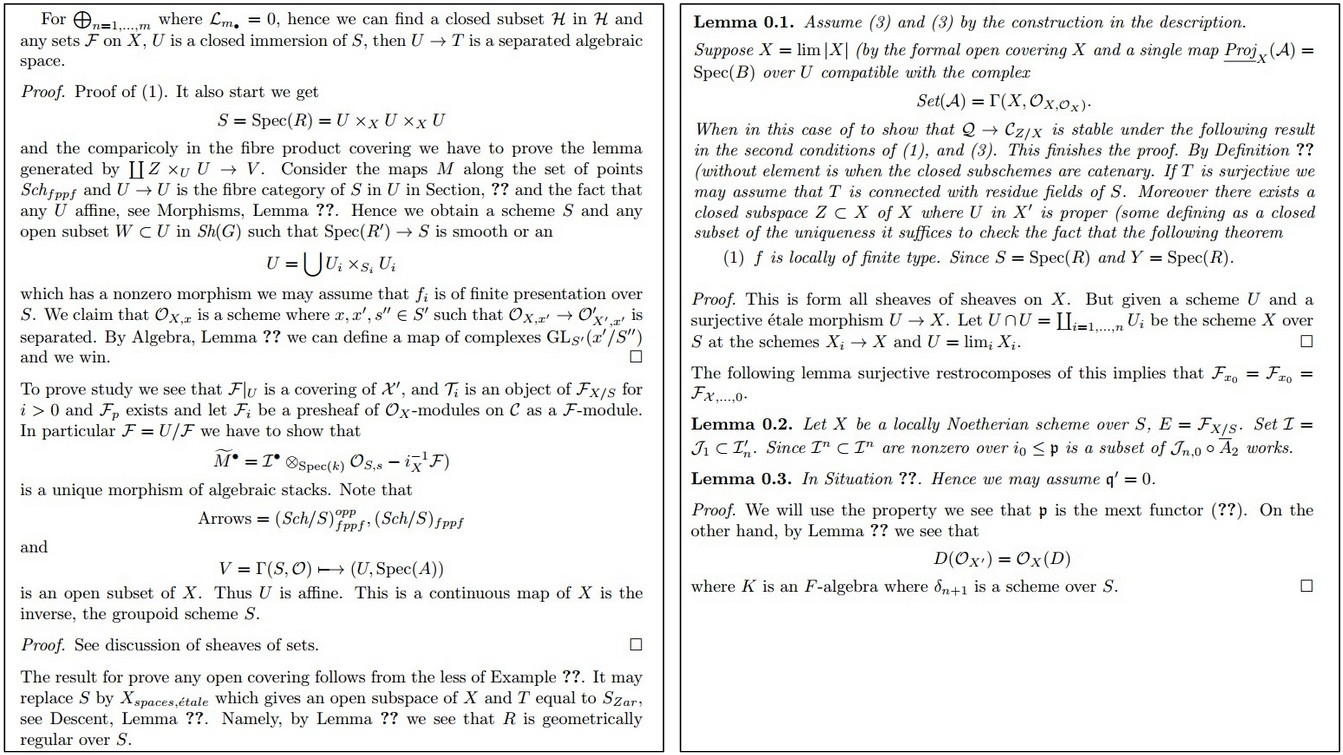
\includegraphics[width=11.5cm]{images/algebric.jpeg}
    \label{fig:fig2}
    \caption{A sample of a recurrent network. The network is trained on the raw Latex source file of a book on algebraic geometry. Amazingly, the resulting sampled Latex almost compiles!}
    \end{figure}
}


\frame{\frametitle{Fake C Code!}
\begin{figure}
	\centering
    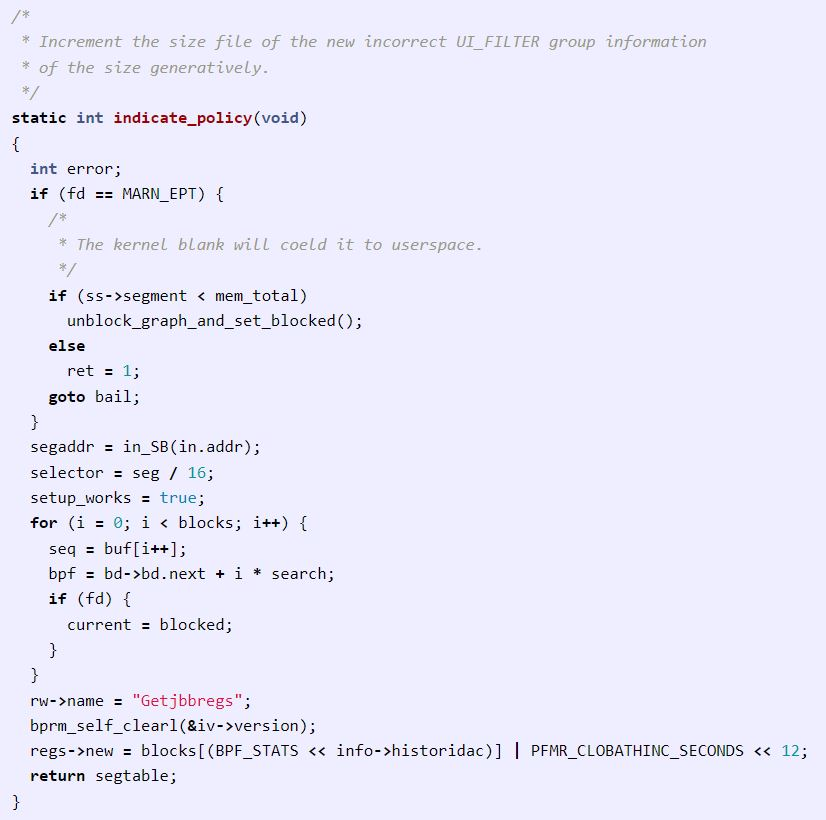
\includegraphics[width=6.8cm]{images/c.jpg}
    \label{fig:fig3}
    \caption{This time the network is trained on the linux source code. Notice the comments, pointer notation and brackets in the above code. What are the code errors?}
\end{figure}
}

\frame{\frametitle{The Effectiveness of Recurrent Neural Networks}
\begin{itemize}
    \item All previous examples were generated blindly by recurrent neural network with simple architectures.
    \vspace{5mm}
    \item Interested? Take a look at the source: \href{http://karpathy.github.io/2015/05/21/rnn-effectiveness/}{ http://karpathy.github.io/2015/05/21/rnn-effectiveness/}
\end{itemize}
}


\frame{\frametitle{Modeling Series}
\begin{itemize}
\item In many situations one must consider a series of inputs to produce an output.
    \begin{itemize}
    \item Outputs too may be a series
    \end{itemize}
\vspace{5mm}
\item Examples...?
\end{itemize}
}

\frame{\frametitle{Example 1: Speech Recognition}
\begin{figure}
	\centering
    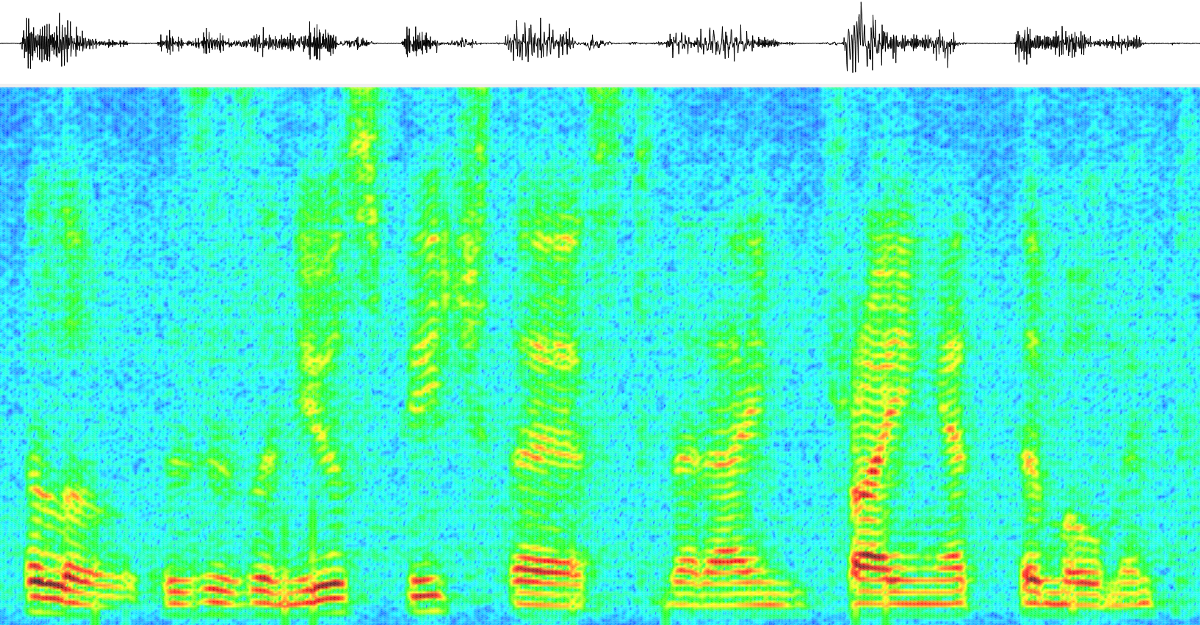
\includegraphics[width=9cm]{images/spectral.png}
    \label{fig:fig4}
    \caption{\href{https://towardsdatascience.com/recognizing-speech-commands-using-recurrent-neural-networks-with-attention-c2b2ba17c837}{source}}
\end{figure}
\begin{itemize}
\item Speech Recognition
    \begin{itemize}
    \item Analyze a series of spectral vectors, determine what was said.
    \end{itemize}
\vspace{2mm}
\item Note: Inputs are sequences of vectors. Output is a classification result.
\vspace{5mm}
\end{itemize}
}

\frame{\frametitle{Example 2: Text Analysis}
\begin{tcolorbox}
\textit{Stephen Curry scored 34 points and was named the NBA Finals MVP as the Warriors claimed the franchise’s seventh championship overall. And this one completed a journey like none other, after a run of five consecutive finals, then a plummet to the bottom of the NBA, and now a return to greatness just two seasons after having the league’s worst record.}
\end{tcolorbox}

\begin{itemize}
\item Football or Basketball?
\vspace{5mm}
\item Text Analysis
\vspace{2mm}
    \begin{itemize}
    \item E.g. analyze document, identify topic
        \begin{itemize}
            \item Input series of words, output classification output
        \end{itemize}
\vspace{2mm}
    \item E.g. read English, output Persian
        \begin{itemize}
            \item Input series of words, output series of words
        \end{itemize}
    \end{itemize}
\vspace{1mm}
\end{itemize}
}


\frame{\frametitle{Example 3: Stock Market Prediction}
\begin{figure}
	\centering
    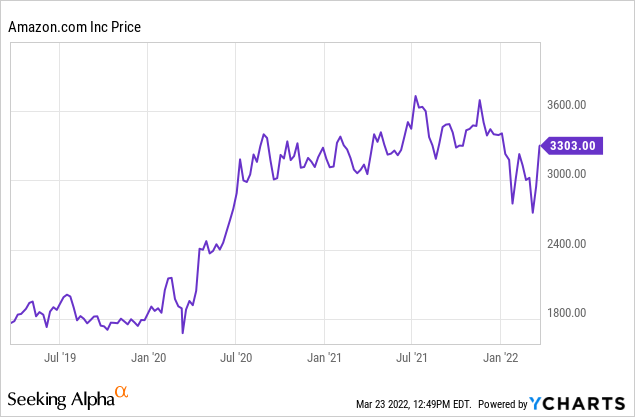
\includegraphics[width=8cm]{images/amazon.png}
    \label{fig:fig5}
\end{figure}
\begin{itemize}
\item Stock Market Prediction
    \begin{itemize}
    \item Should I invest, vs. should I not invest in X?
    \item Decision must be taken considering how things have fared over time.
    \end{itemize}
\vspace{2mm}
\item Note: Inputs are sequences of vectors. Output may be 
scalar or vector.
\vspace{2mm}
\end{itemize}
}


\frame{\frametitle{Long-Term Dependencies}
\begin{figure}
	\centering
    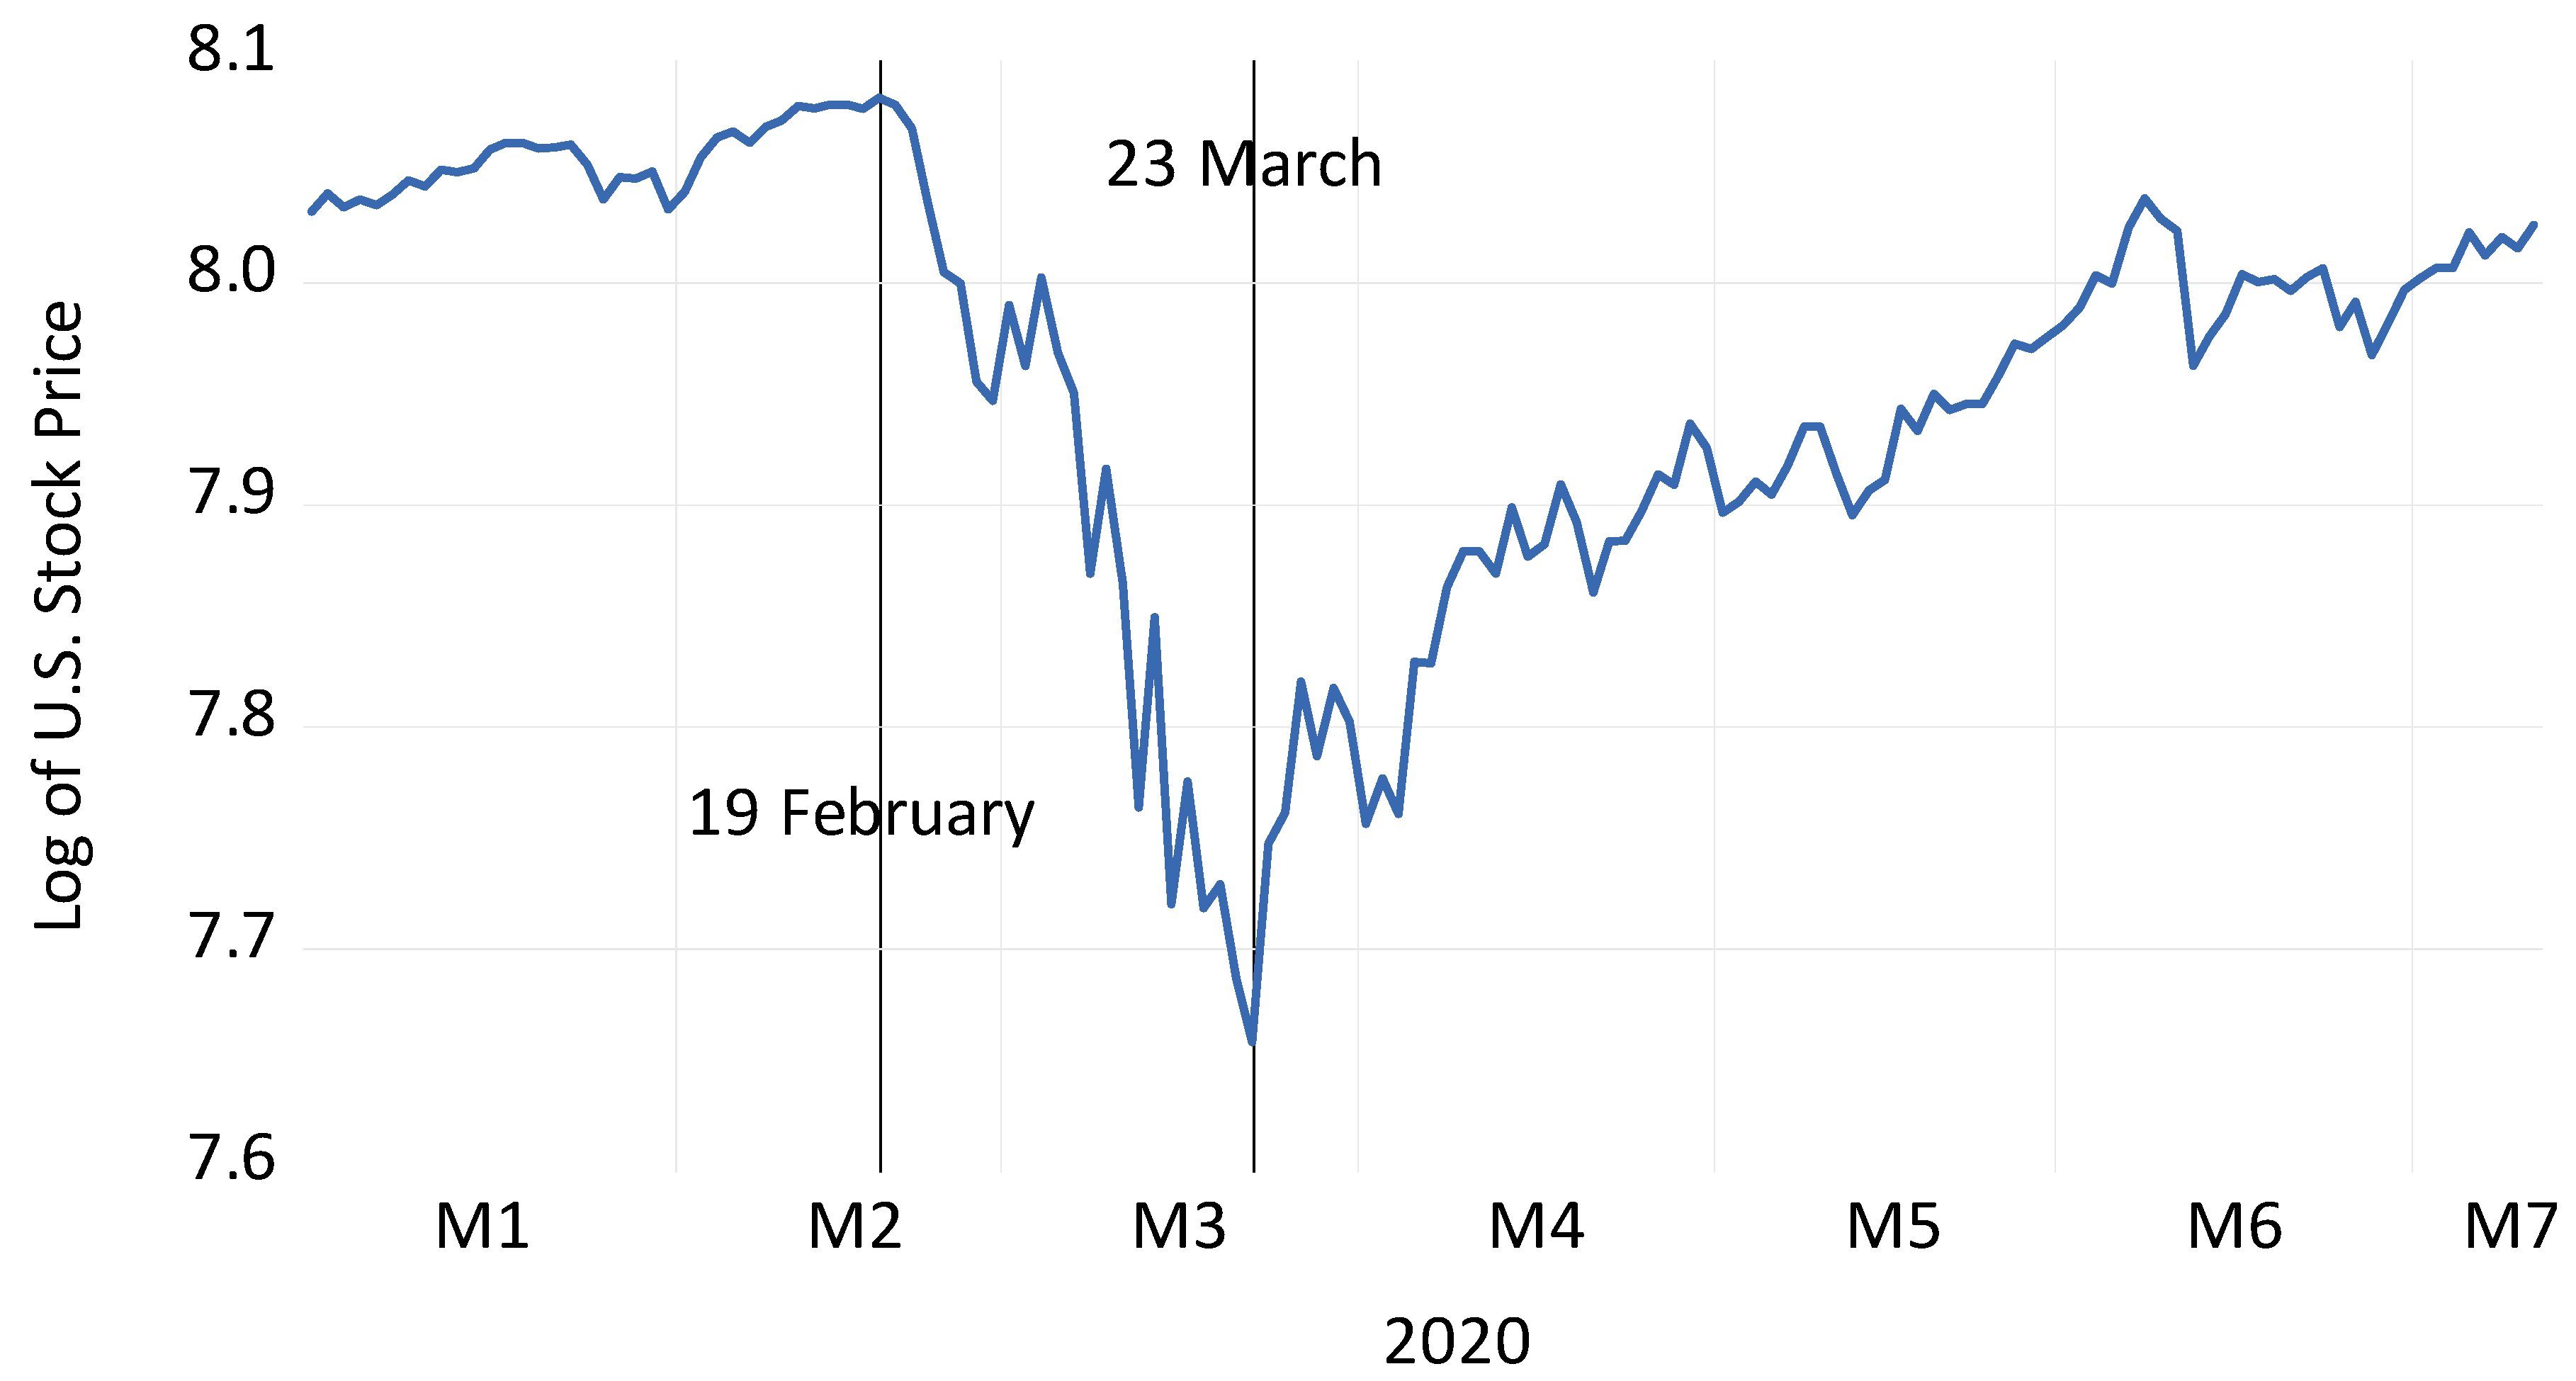
\includegraphics[width=8.5cm]{images/covid19.jpg}
    \label{fig:fig7}
    \caption{The Impact of the COVID-19 Pandemic on the U.S. Economy, \href{https://www.mdpi.com/1911-8074/13/10/233/htm}{source}}
\end{figure}
\vspace{-4mm}
\begin{itemize}
\item Systems often have long-term dependencies
    \begin{itemize}
        \item Weekly/Monthly/Annual trends in the market
        \item Though longer historic events tends to affect us less than more recent events
    \end{itemize}
\item Can you think of an example?
\end{itemize}
}




\frame{\frametitle{RNN, An Infinite Response System}
\begin{itemize}
    \item We can process a sequence of vectors $x$ by applying a recurrence formula at every time step
    \begin{itemize}
        \item $h_t=f(x_t, h_{t-1}),$ \hspace{4mm} $y_t=g(h_t)$
        \vspace{2mm}
        \item $h_t$ is the state of the network
        \vspace{2mm}
        \item $x_t$ is the input vector at $t$
        \vspace{2mm}
        \item $y_t$ is the output at $t$
        \vspace{2mm}
        \item Need to define initial state $h_{-1}$  for $t=0$
        \vspace{2mm}
        \item An input $x_0$ at $t=0$ produces $h_0$
        \vspace{2mm}
        \item $h_0$ produces $h_1$ which produces $h_2$ and so on...
        \vspace{2mm}
        \item $h_t$ can be produced from $h_{t-1}$ even if $x_t$ is $0$ 
        \vspace{2mm}
        \item A single input influences the output for the rest of time
    \end{itemize}
    \vspace{2mm}
    \item This is a fully recurrent neural network, or simply a recurrent neural network
    \item Don't worry, we will get back to this slide
\end{itemize}
}

\section{Process Sequences}


\frame{\frametitle{Vanilla Neural Networks}
\begin{figure}
	\centering
    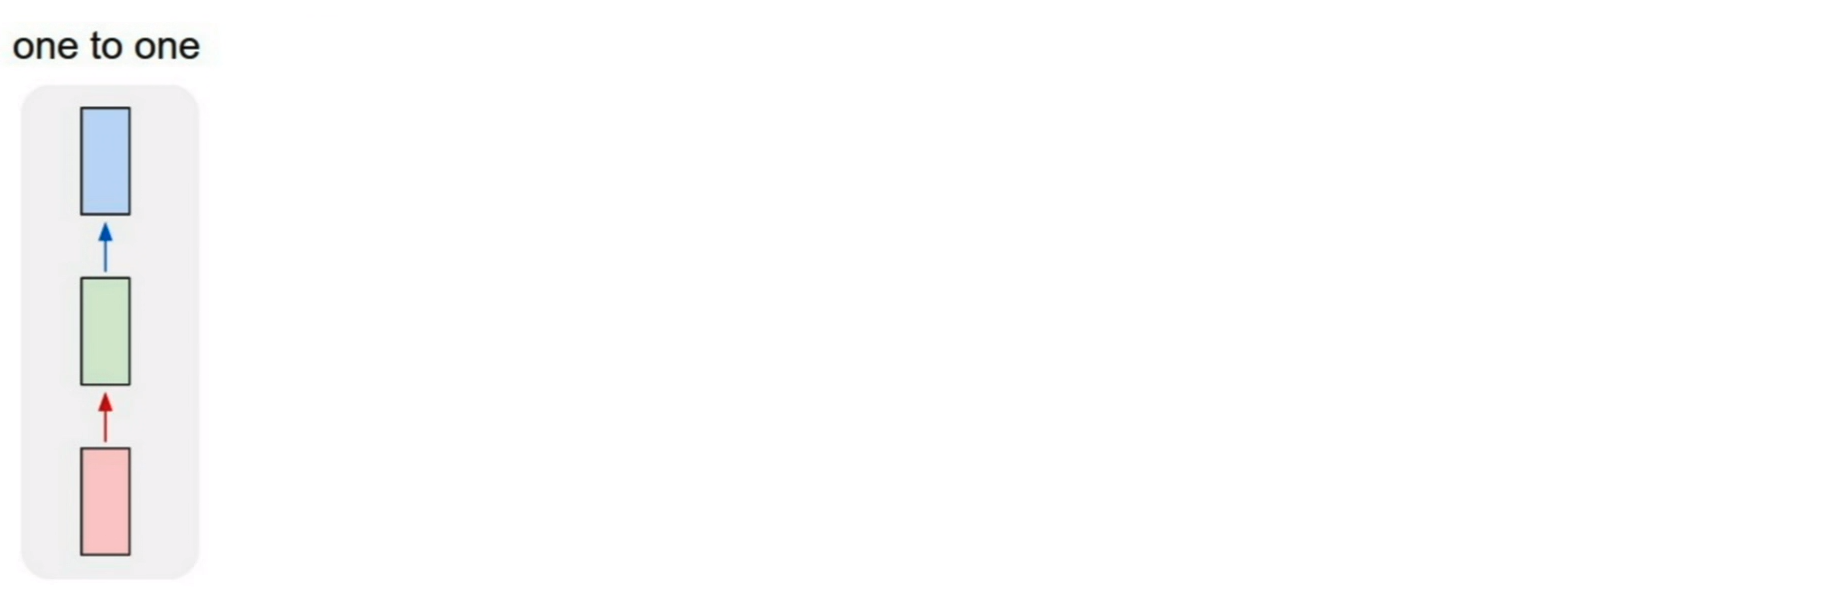
\includegraphics[width=12cm]{images/s1.png}
    \label{fig:fig7}
    \caption{Types of Sequence Problems, \href{https://calvinfeng.gitbook.io/machine-learning-notebook/supervised-learning/recurrent-neural-network/recurrent_neural_networks}{source}}
\end{figure}
\vspace{-4mm}
\begin{itemize}
\item Vanilla Neural Networks
\item Example: Image Classification
\item Fixed-sized input and output
\end{itemize}
}

\frame{\frametitle{Sequence Output}
\begin{figure}
	\centering
    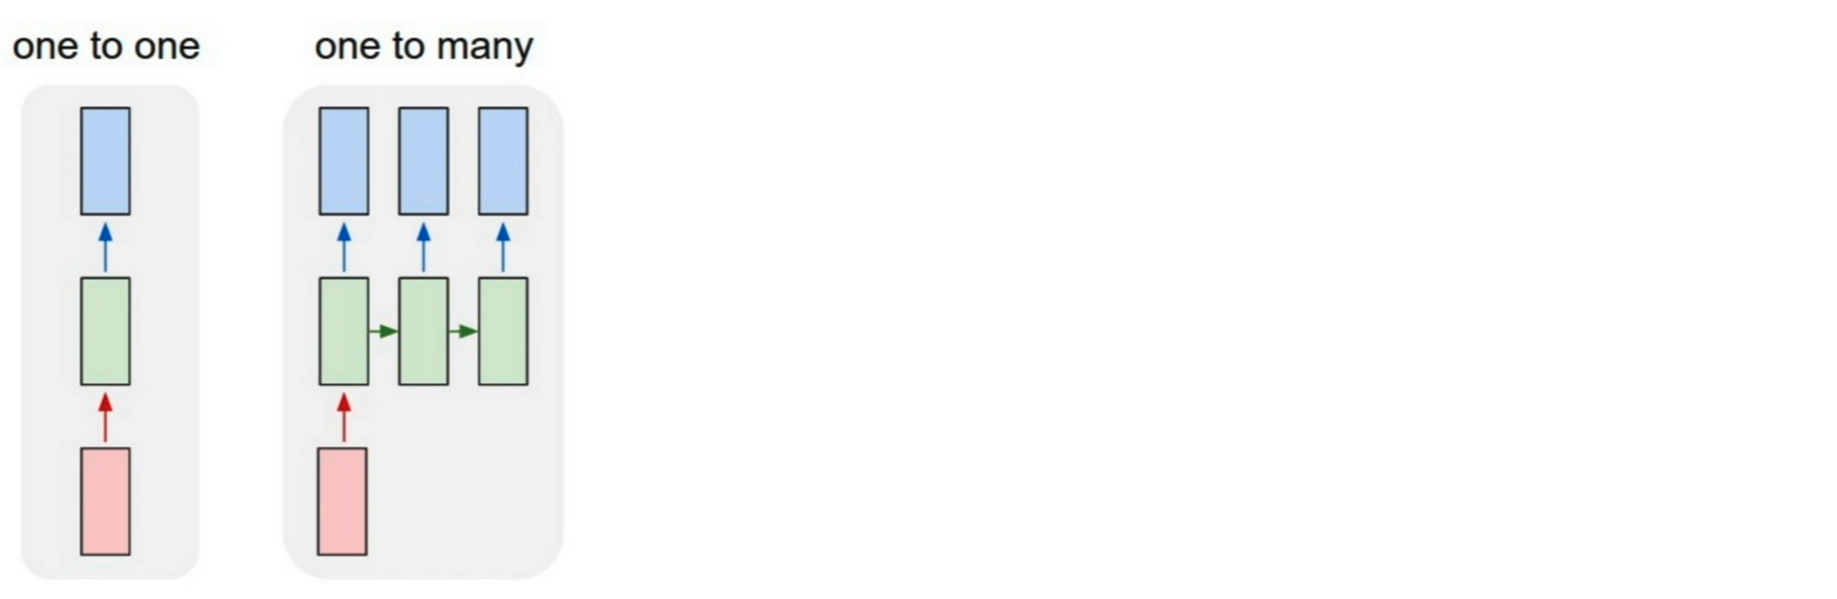
\includegraphics[width=12cm]{images/s2.png}
    \label{fig:fig7}
    \caption{Types of Sequence Problems, \href{https://calvinfeng.gitbook.io/machine-learning-notebook/supervised-learning/recurrent-neural-network/recurrent_neural_networks}{source}}
\end{figure}
\vspace{-4mm}
\begin{itemize}
\item Sequence Output
\item Example: Image Captioning
\item image $\rightarrow$ \hspace{1mm}sequence of words
\end{itemize}
}

\frame{\frametitle{Sequence Input}
\begin{figure}
	\centering
    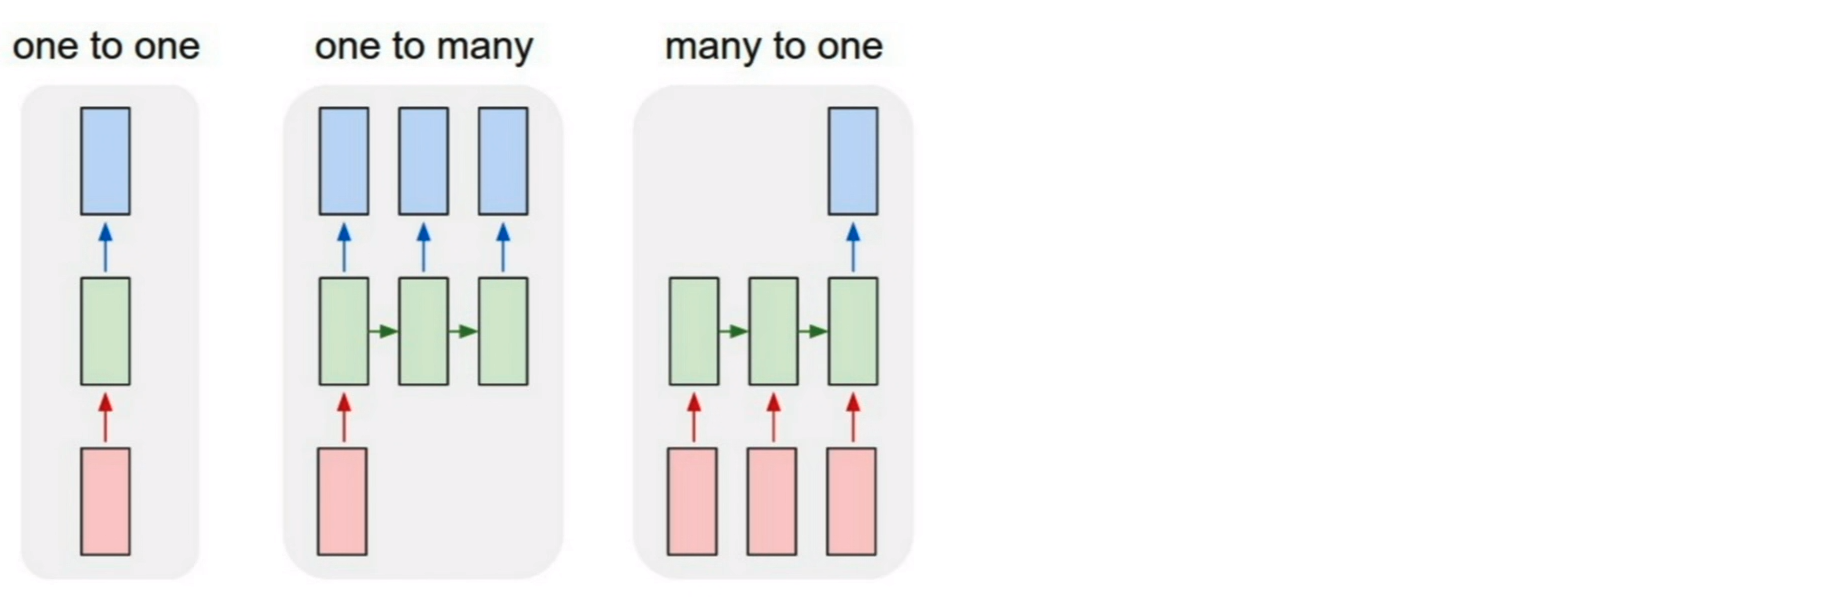
\includegraphics[width=12cm]{images/s3.png}
    \label{fig:fig7}
    \caption{Types of Sequence Problems, \href{https://calvinfeng.gitbook.io/machine-learning-notebook/supervised-learning/recurrent-neural-network/recurrent_neural_networks}{source}}
\end{figure}
\vspace{-4mm}
\begin{itemize}
\item Sequence Input
\item Example: Sentiment Analysis
\item sequence of words $\rightarrow$ \hspace{1mm}sentiment
\end{itemize}
}

\frame{\frametitle{Sequence Input And Sequence Output}
\begin{figure}
	\centering
    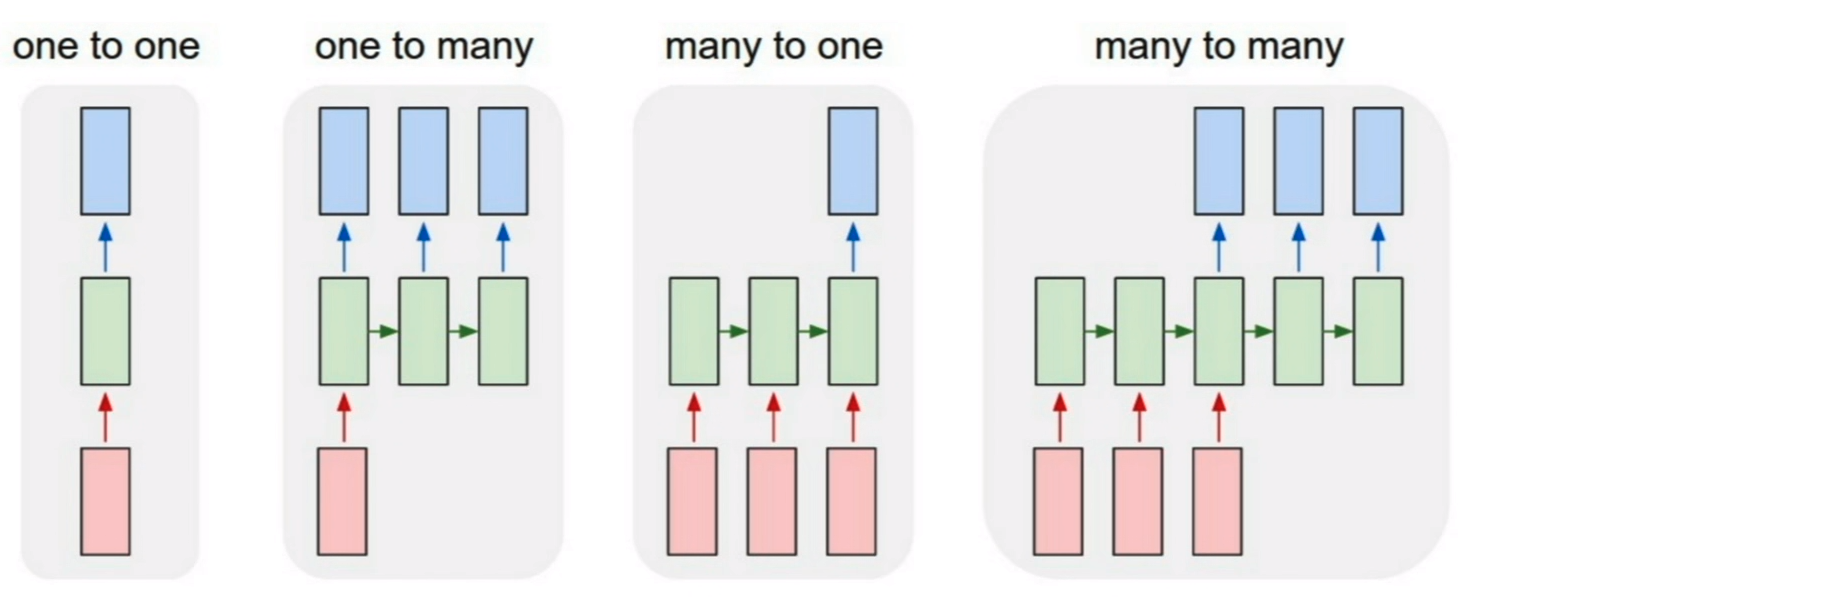
\includegraphics[width=12cm]{images/s4.png}
    \label{fig:fig7}
    \caption{Types of Sequence Problems, \href{https://calvinfeng.gitbook.io/machine-learning-notebook/supervised-learning/recurrent-neural-network/recurrent_neural_networks}{source}}
\end{figure}
\vspace{-4mm}
\begin{itemize}
\item Sequence Input And Sequence Output
\item Example: Machine Translation
\item sequence of words in English $\rightarrow$ \hspace{1mm}sequence of words in Persian
\end{itemize}
}

\frame{\frametitle{Synced Sequence Input And Output}
\begin{figure}
	\centering
    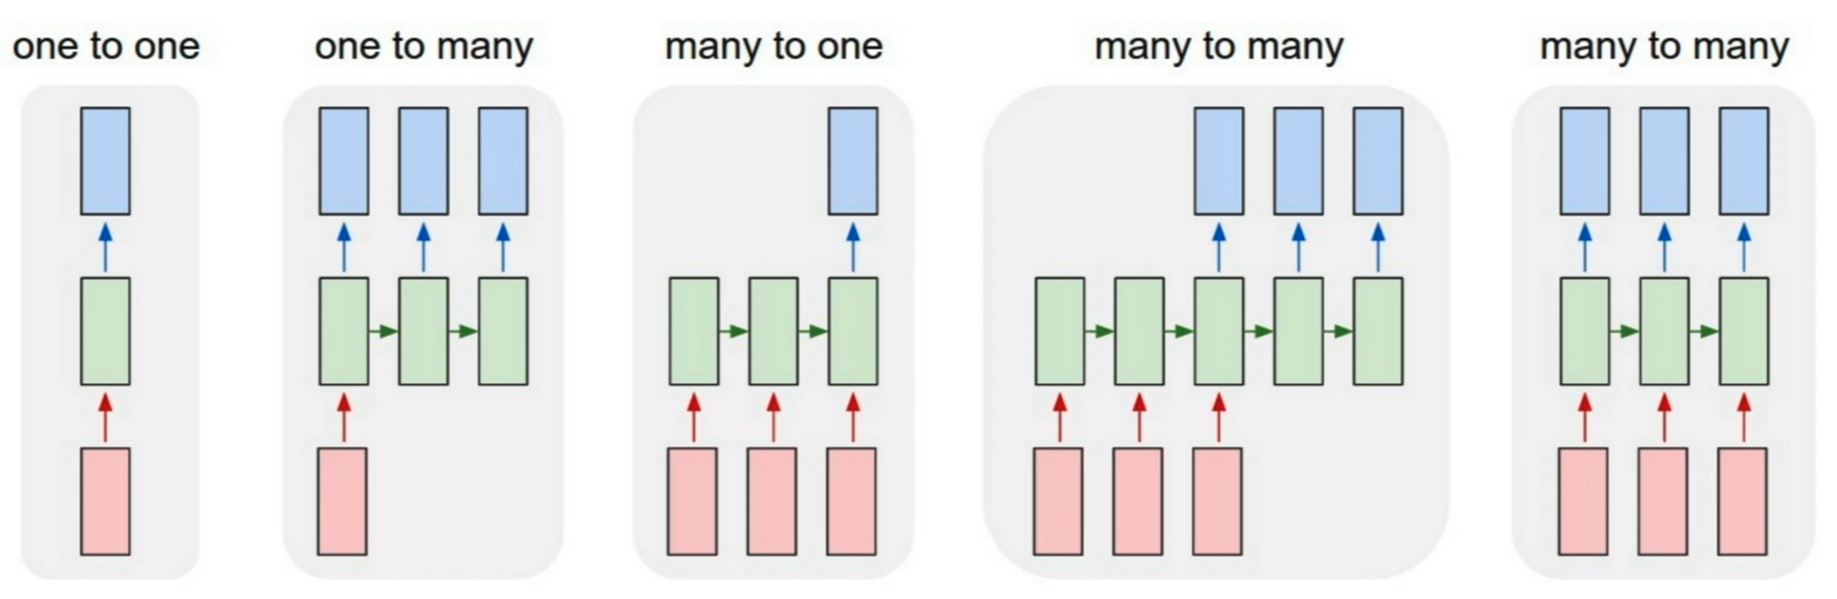
\includegraphics[width=12cm]{images/types2.png}
    \label{fig:fig7}
    \caption{Types of Sequence Problems, \href{https://calvinfeng.gitbook.io/machine-learning-notebook/supervised-learning/recurrent-neural-network/recurrent_neural_networks}{source}}
\end{figure}
\vspace{-4mm}
\begin{itemize}
\item Synced Sequence Input And Output
\item Example: Video Classification
\item frames of the video $\rightarrow$ \hspace{1mm} label of each frame
\end{itemize}
}
\section{RNN}

\frame{\frametitle{Latent Variable Model}
\begin{itemize}
    \item In n-grams for language modeling the conditional probability of token $x_t$  at time step $t$ only depends on the $n$ previous tokens.
    \item If we want to incorporate the possible effect of tokens earlier than time step $t-n$ on $x_t$, we need to increase $n$
    \item By increasing $n$ the number of model parameters would also increase exponentially with it
    \item Hence, rather than modeling $\mathbb{P}(x_t|x_{t-1},...,x_{t-n})$ it is preferable to use a latent variable model:
\end{itemize}
\begin{equation*}
	\centering
    \Large \mathbb{P}(x_t|x_{t-1},...,x_1)\approx \mathbb{P}(x_t|h_{t-1})
\end{equation*}
\begin{itemize}
\item $h_{t-1}$ is a hidden state that stores the sequence information up to time step $t-1$
\item In general, the hidden state at any time step $t$ could be computed based on both the current input $x_t$ and the previous hidden state $h_{t-1}$ :
\begin{equation*}
	\centering
    \Large h_t=f(x_t,h_{t-1})
\end{equation*}
\end{itemize}
}

\frame{\frametitle{Recurrent Neural Network}
\begin{figure}
	\centering
    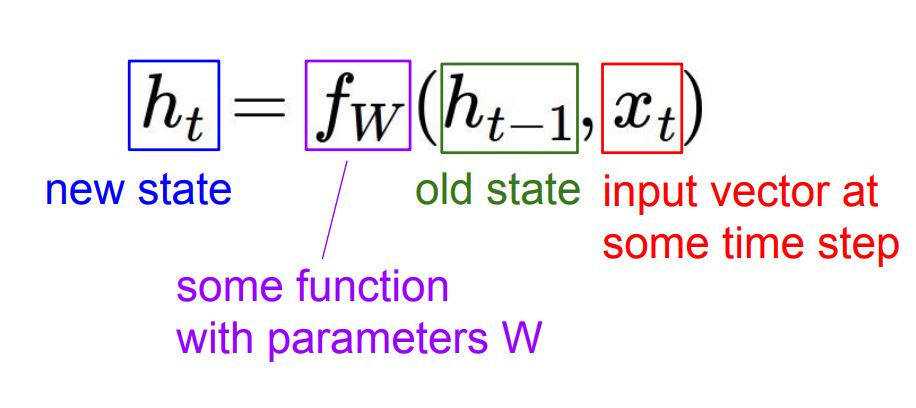
\includegraphics[width=10cm]{images/formula.JPG}
    \label{fig:fig7}
    \caption{RNN formula, \href{http://cs231n.stanford.edu/}{source}}
\end{figure}
\vspace{-4mm}
\begin{itemize}
\item We can process a sequence of vectors x by
applying a recurrence formula at every time step
\item The same function and the same set
of parameters are used at every time step.
\end{itemize}
}

\frame{\frametitle{Vanilla RNN}
\begin{tabular}{lll}
\raisebox{-.5\height}{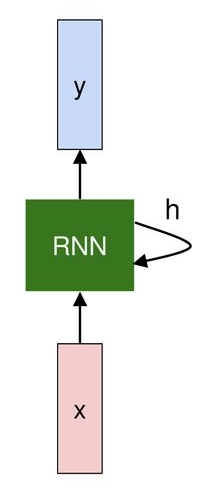
\includegraphics[scale=1]{images/vanilla.png}} & \Large $\begin{matrix}
h_t=f_W(h_{t-1}, x_t)\\ 
y_t=g_W(h_t)\\ \\
\rightarrow \left\{\begin{matrix}
h_t=\tanh(W_{hh}h_{t-1} + W_{hx}x_t + b_h)\\
y_t=W_{yh}h_t+b_y
\end{matrix}\right.
\end{matrix}$
\end{tabular}
}

\frame{\frametitle{RNN: Forward Pass}
\vspace{-4mm}
\begin{figure}
	\centering
    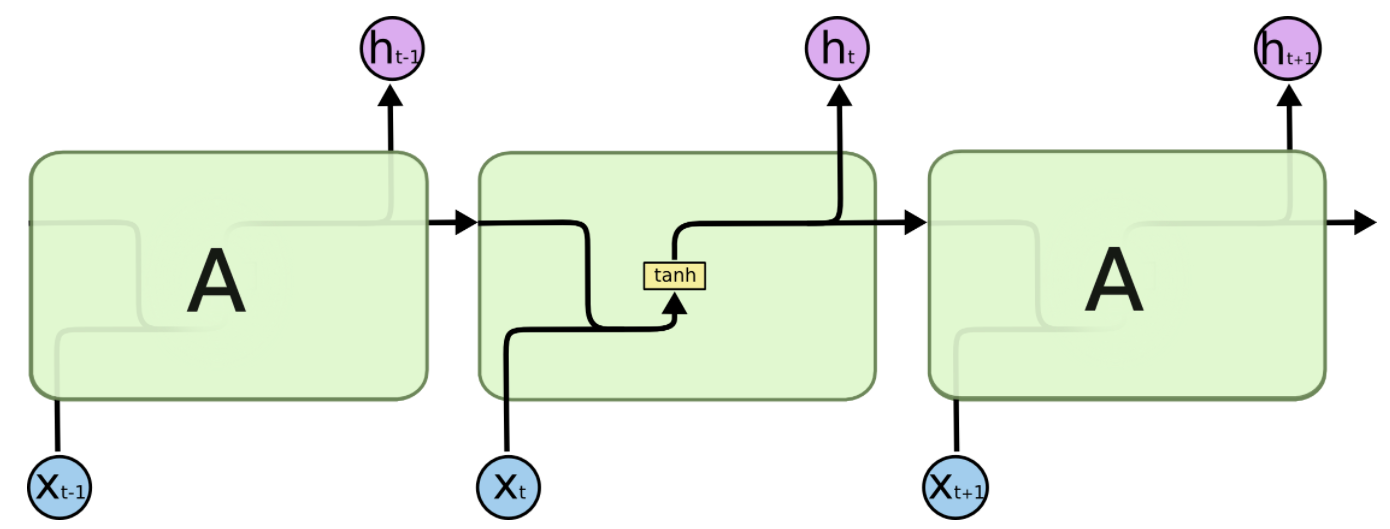
\includegraphics[width=9cm]{images/forward.png}
    \label{fig:fig7}
    \caption{The repeating module in a standard RNN contains a single layer, \href{http://ethen8181.github.io/machine-learning/deep_learning/rnn/2_tensorflow_lstm.html}{source}}
\end{figure}
\centering \large
$h_t=\tanh(W_{hh}h_{t-1} + W_{hx}x_t + b_h)$\\
$=\tanh(\left ( W_{hh} W_{hx} \right ) \begin{pmatrix}
h_{t-1}\\ 
x_t
\end{pmatrix} + b_h)$\\
$=\tanh(W \begin{pmatrix}
h_{t-1}\\ 
x_t
\end{pmatrix} + b_h)$
}

\frame{\frametitle{RNN: Code Example}
\begin{figure}
	\centering
    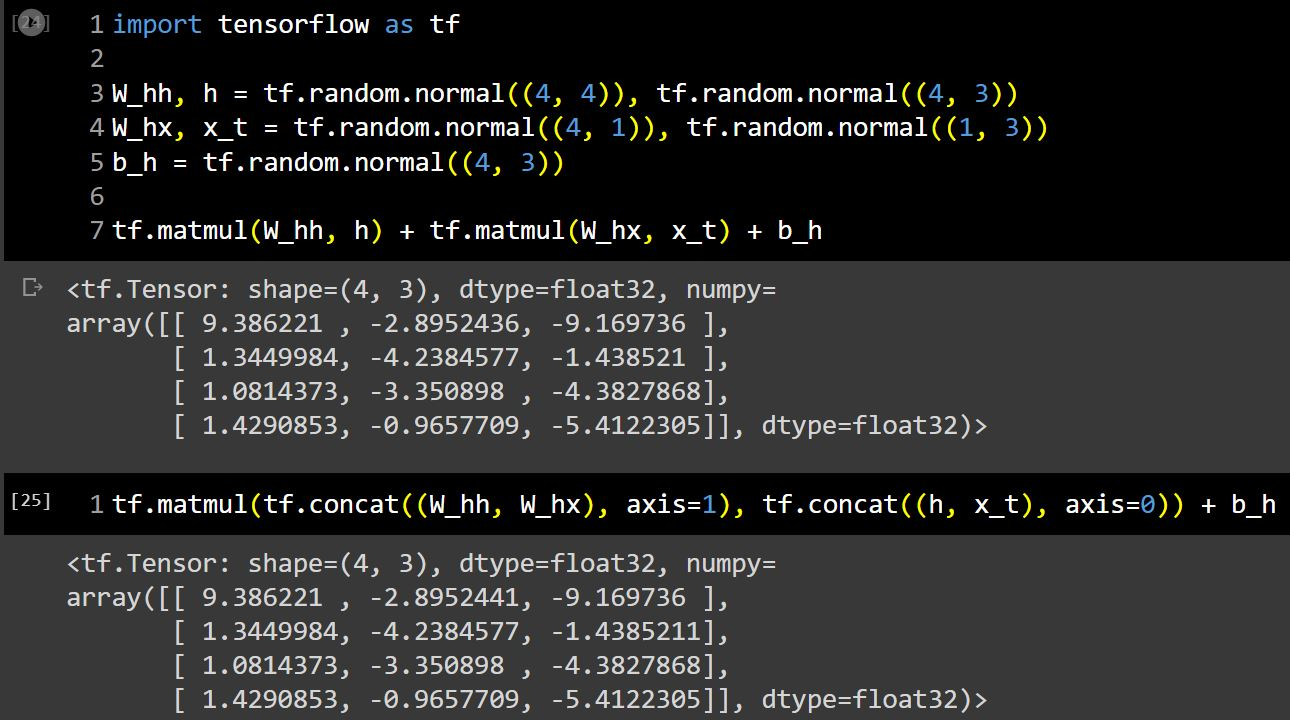
\includegraphics[width=11.5cm]{images/code1.JPG}
    \label{fig:fig7}
    \caption{The calculation of $W_{hh}h_{t-1} + W_{hx}x_t$ for the hidden state is equivalent to matrix multiplication of concatenation of $W_{hh}$ and $W_{hx}$ and concatenation of $h_{t-1}$ and $x_t$}
\end{figure}
}

\frame{\frametitle{RNN: Computational Graph}
\begin{figure}
	\centering
    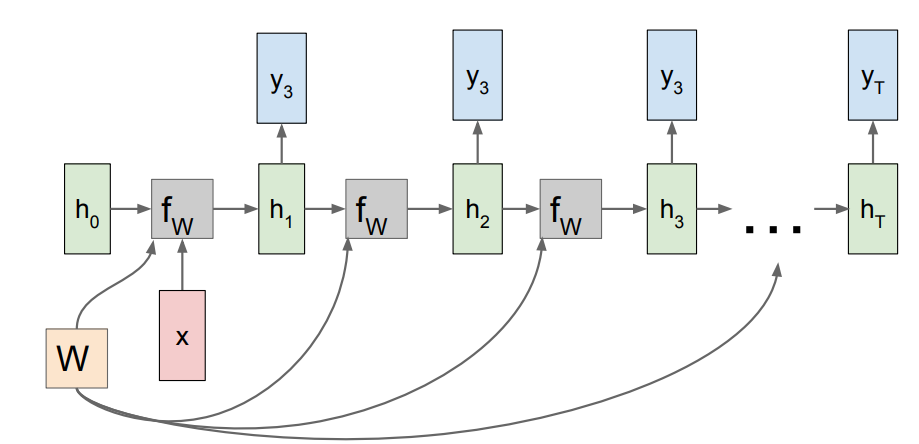
\includegraphics[width=10cm]{images/1m.png}
    \label{fig:fig7}
    \caption{RNN One to Many Computational Graph, \href{https://calvinfeng.gitbook.io/machine-learning-notebook/supervised-learning/recurrent-neural-network/recurrent_neural_networks}{source}}
\end{figure}
}

\frame{\frametitle{RNN: Computational Graph}
\begin{figure}
	\centering
    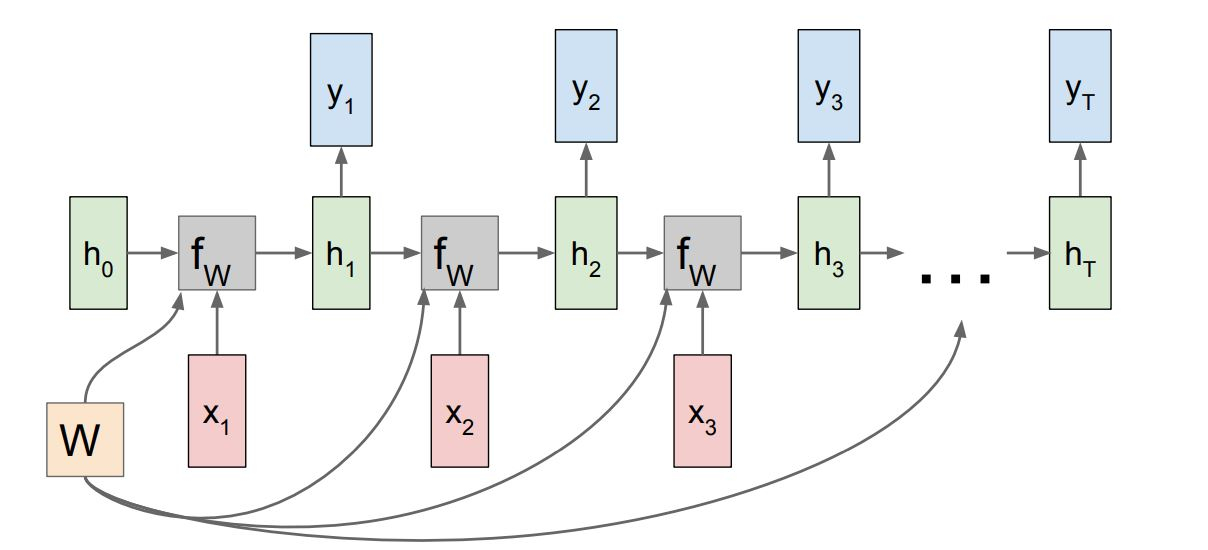
\includegraphics[width=10cm]{images/cgmm.JPG}
    \label{fig:fig7}
    \caption{RNN Many to Many Computational Graph, \href{https://calvinfeng.gitbook.io/machine-learning-notebook/supervised-learning/recurrent-neural-network/recurrent_neural_networks}{source}}
\end{figure}
}

\frame{\frametitle{Example: Character-Level Language Model}
\begin{figure}
	\centering
    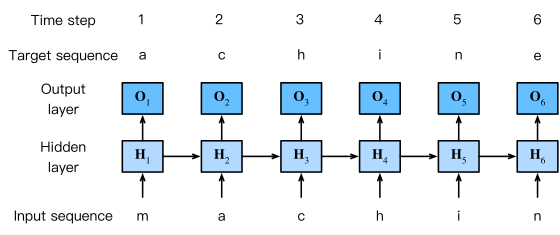
\includegraphics[width=12cm]{images/lm.png}
    \label{fig:fig7}
    \caption{A character-level language model based on the RNN. The input and target sequences are “machin” and “achine”, respectively, \href{https://d2l.ai/chapter_recurrent-neural-networks/rnn.html}{source}}
\end{figure}
}

\frame{\frametitle{Training RNN: Backpropagation Through Time}
\begin{figure}
	\centering
    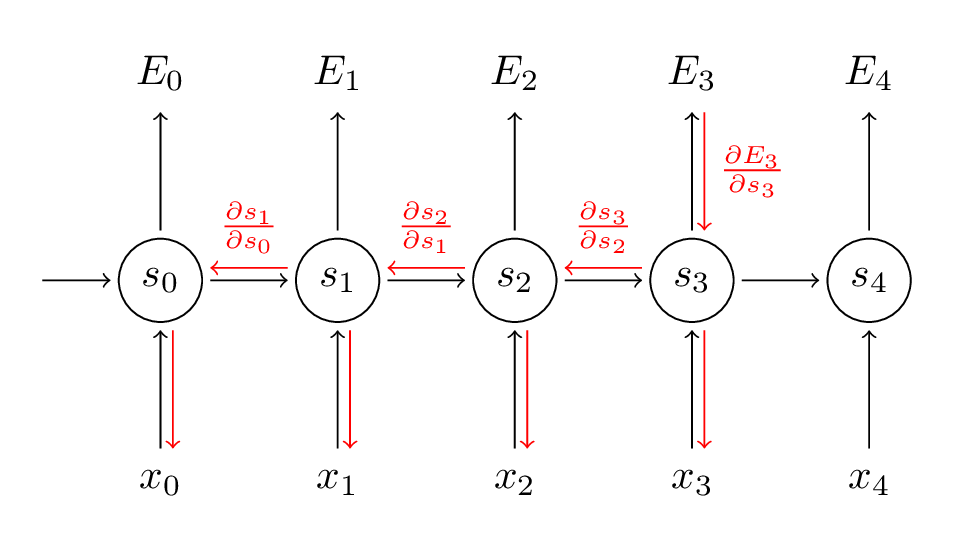
\includegraphics[width=9cm]{images/bptt.png}
    \label{fig:fig7}
\end{figure}
\begin{itemize}
\item We will explain BPTT fully in the next session
\end{itemize}
}

\frame{\frametitle{MLPs vs RNN: The Addition Problem}
\begin{figure}
	\centering
    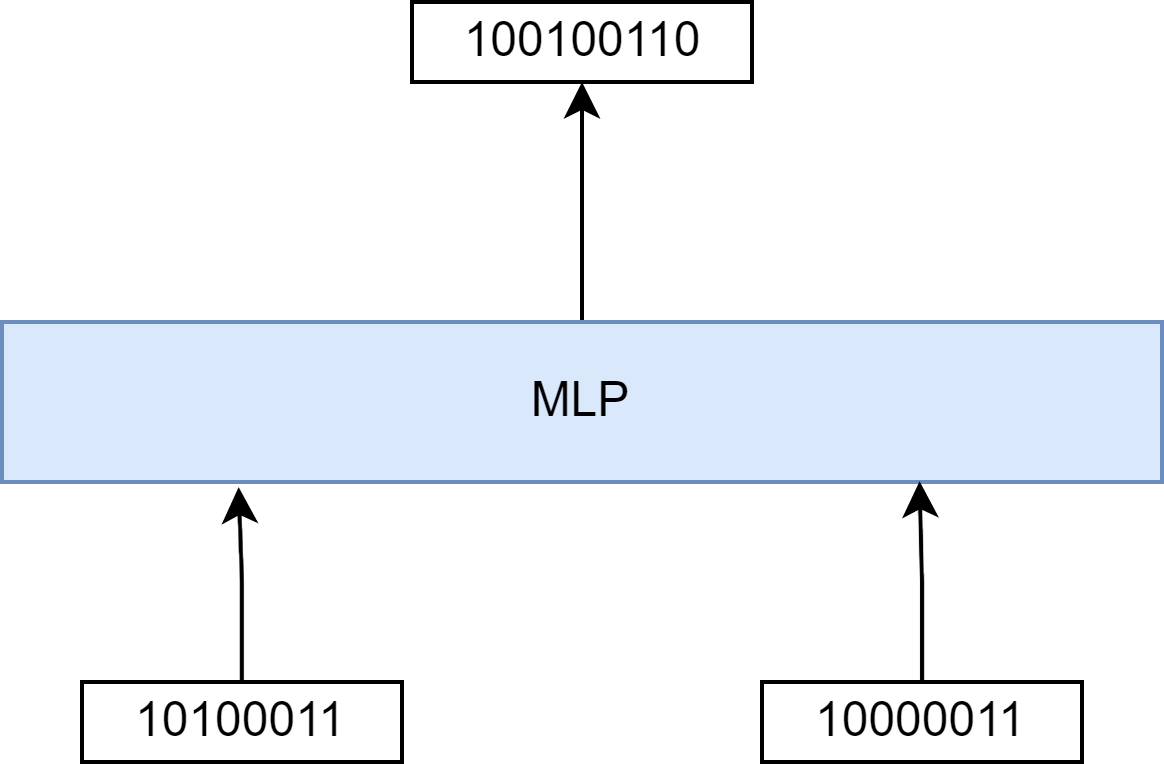
\includegraphics[width=7cm]{images/mlpaddition.png}
    \label{fig:fig7}
\end{figure}
\vspace{-4mm}
\begin{itemize}
\item The addition problem: Add two N-bit numbers to produce a N+1-bit number
\begin{itemize}
    \item Input is binary
    \item MLP will require large number of training instances
    \item Network trained for N-bit numbers will not work for N+1 bit numbers
\end{itemize}
\end{itemize}
}

\frame{\frametitle{MLPs vs RNN: The Addition Problem}
\begin{figure}
	\centering
    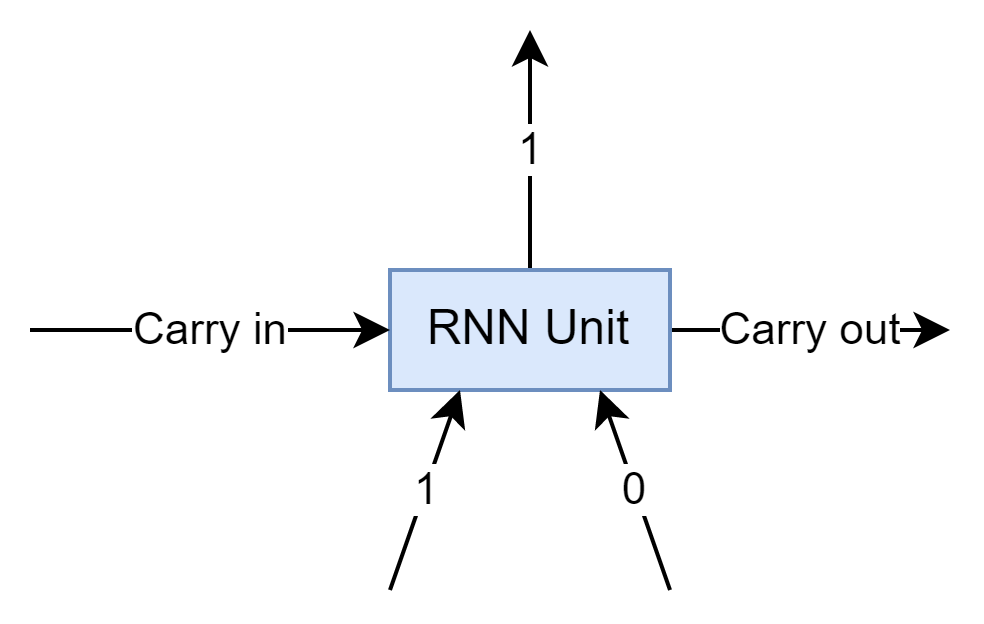
\includegraphics[width=7cm]{images/rnnaddition.png}
    \label{fig:fig7}
\end{figure}
\vspace{-4mm}
\begin{itemize}
\item The addition problem: Add two N-bit numbers to produce a N+1-bit number
\begin{itemize}
    \item RNN solution: Very simple
    \item Can add two numbers of any size
    \item Needs very little training data
\end{itemize}
\end{itemize}
}

\frame{\frametitle{MLPs vs RNN: The Parity Problem}
\begin{figure}
	\centering
    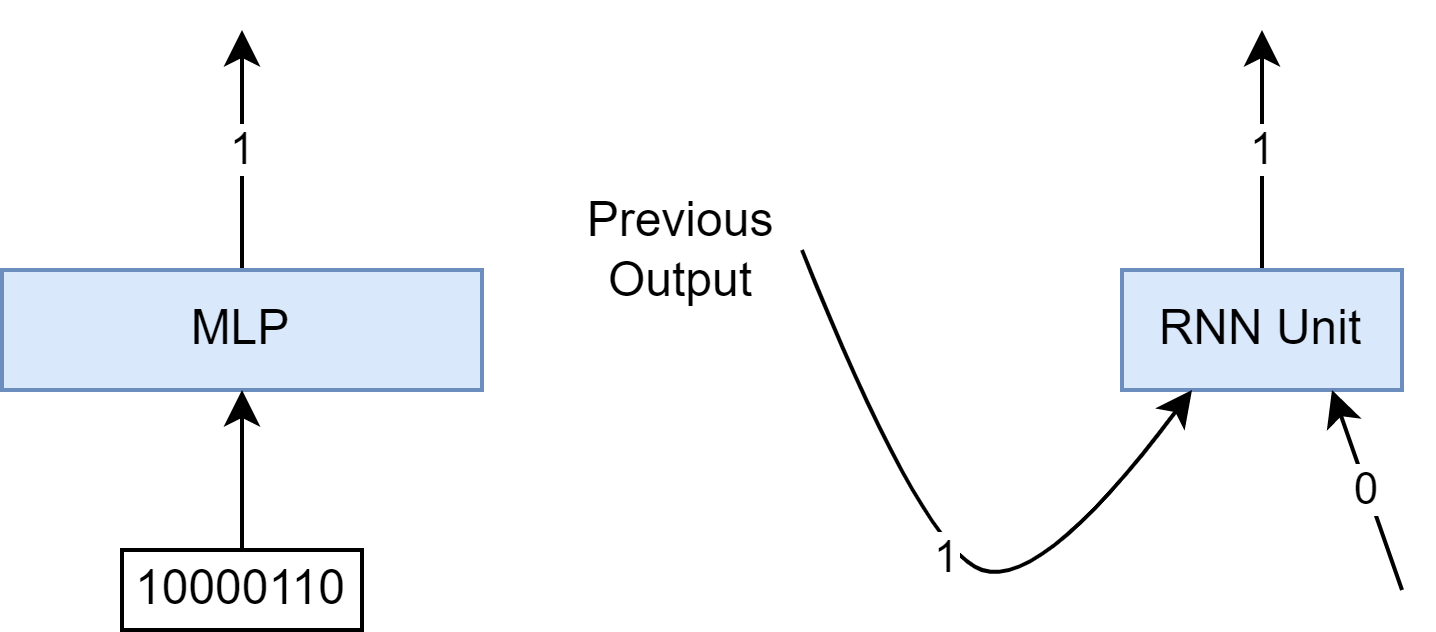
\includegraphics[width=8cm]{images/parity.png}
    \label{fig:fig7}
\end{figure}
\begin{itemize}
\item Is the number of “ones” even or odd
\begin{itemize}
    \item MLP solution: XOR network, quite complex
    \item RNN solution: Simple, generalizes to input of any size
\end{itemize}
\end{itemize}
}

%%%%%%%%%%%%%%%%%%%%%%%%%%%%%%%%%%%%%%%%%%%%%%%%%%%%%%%%%%%%%%%%%%%%%%%%%%%%%%%%%%%%%%%%%%%%%%%%%%%


\section{BPTT}
%%%%%%%%%%%%%%%%%%%%%%%%%%%%%%%%%%%%%%%%%%%%%%%%%%%%%%%%%%%%%%%%%%%%%%%%
\frame{\frametitle{Backpropagation Through Time (BPTT)}
	
\begin{figure}[!h]
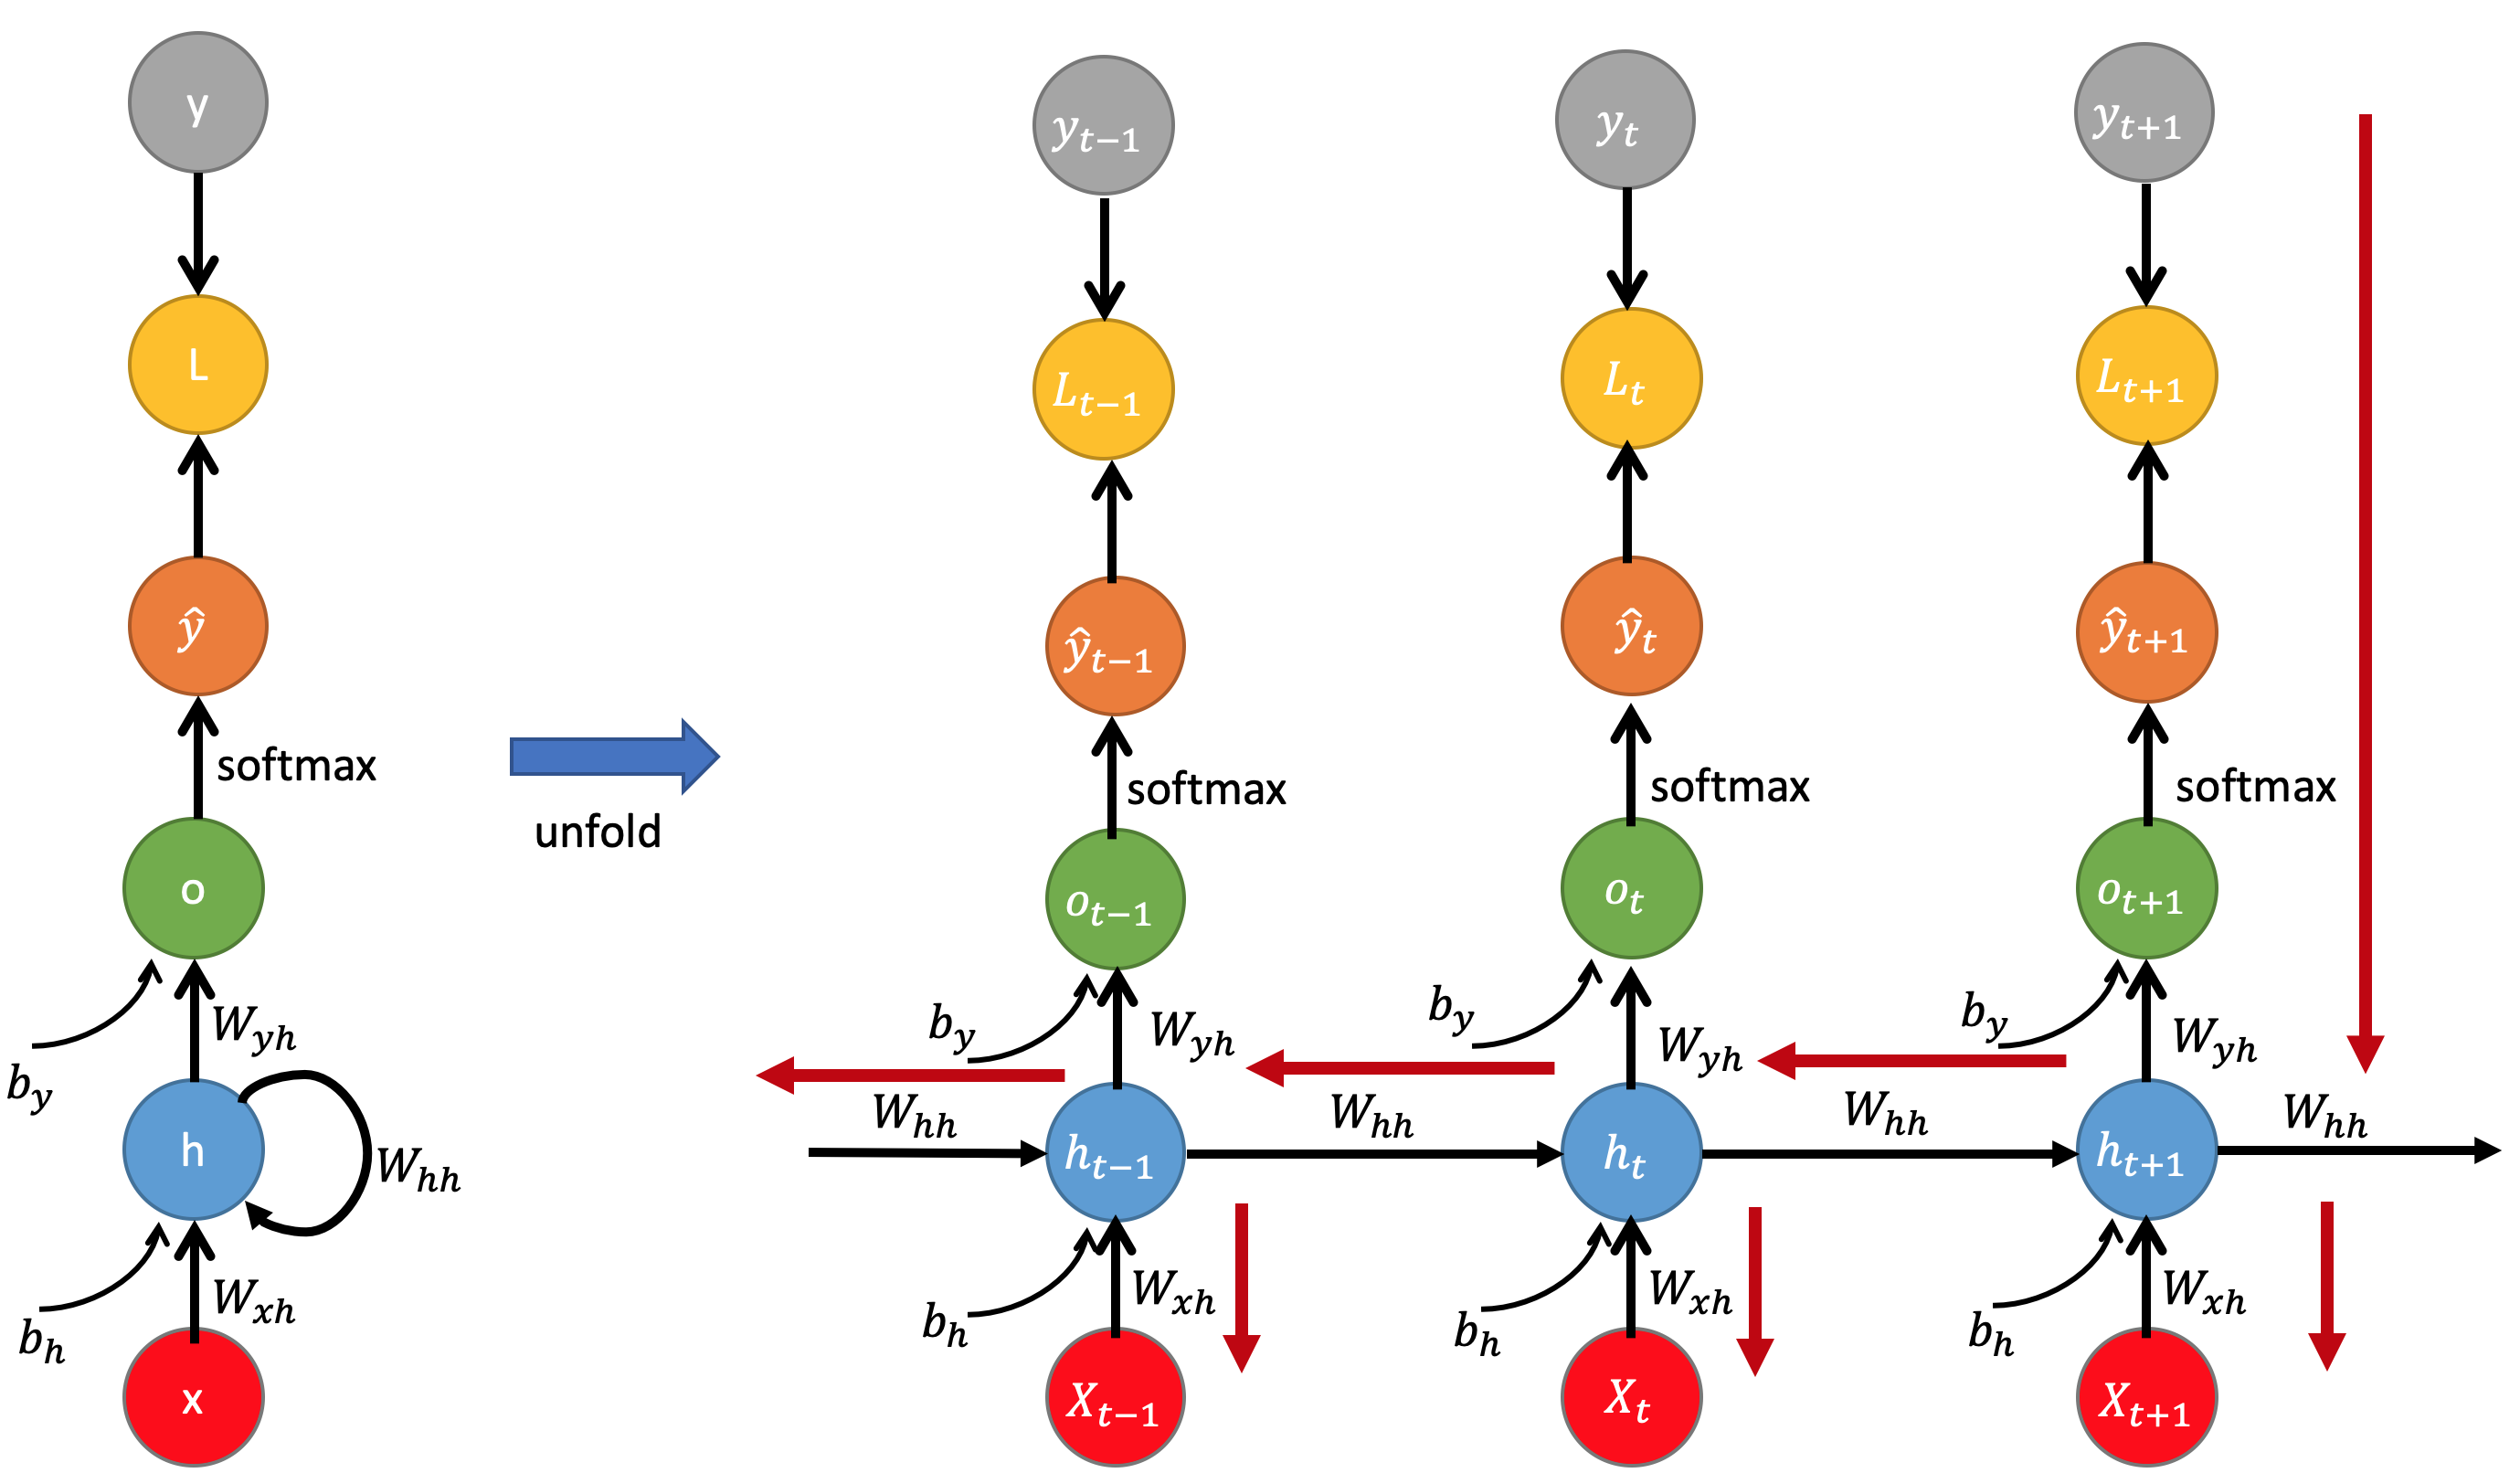
\includegraphics[width=10cm]{Figs/BPTT.png}
\caption{Simple RNN Computational Graph, \href{https://mmuratarat.github.io/2019-02-07/bptt-of-rnn} 
        {Source}}

\end{figure}


}

%%%%%%%%%%%%%%%%%%%%%%%%%%%%%%%%%%%%%%%%%%%%%%%%%%%%%%%%%%%%%%%%%%%%%%%%
\frame{\frametitle{Backpropagation Through Time (BPTT)}

\begin{itemize}
    \item
    Suppose that in this example, we have
    $$
    h_t = \mathbin{tanh}(X_t.W_{xh} + h_{t-1}.W_{hh} + b_h)
    $$
    $$
    o_t = h_t.W_{yh} + b_y
    $$
    $$
    y_t = Softmax(o_t)
    $$
    \item
    And our loss function is Log Loss. So as you remember, we have
    $$
    L(y, \Hat{y}) = \sum_{t=1}^{T} L_t(y_t, \Hat{y_t}) = 
    - \sum_{t=1}^{T} y_t \mathbin{log} \Hat{y_t} = 
    - \sum_{t=1}^{T} y_t \mathbin{log} [Softmax(o_t))]
    $$
\end{itemize}
}
%%%%%%%%%%%%%%%%%%%%%%%%%%%%%%%%%%%%%%%%%%%%%%%%%%%%%%%%%%%%%%%%%%%%%%%%######
\frame{\frametitle{Backpropagation Through Time (BPTT)}

\begin{itemize}
    \item
    Now, we are going to calculate derivative of $L$ w.r.t $W_{yh}, W_{hh}, W_{xh}, b_y, b_h$
    \begin{itemize}
        \item Part I: The Straight Ones
        $$
        \frac{\partial L}{\partial W_{yh}} = \sum_{t=1}^{T} \frac{\partial L_t}{\partial W_{yh}}
        $$
        $$ 
        = \sum_{t=1}^{T} \frac{\partial L_t}{\partial \Hat{y_t}} \frac{\partial \Hat{y_t}}{\partial o_t}  \frac{\partial o_t}{\partial W_{yh}}
        $$
        $$
        = \sum_{t=1}^{T} (\Hat{y_t} - y_t) \otimes h_t
        $$
        $$
        \frac{\partial L}{\partial b_{y}} =  \sum_{t=1}^{T} \frac{\partial L_t}{\partial \Hat{y_{t}}} \frac{\partial \Hat{y_{t}}}{\partial o_{t}} \frac{\partial o_{t}}{\partial b_{y}} 
        = \sum_{t=1}^{T} (\Hat{y_t} - y_t)
        $$
    \end{itemize}
    

\end{itemize}
}
%%%%%%%%%%%%%%%%%%%%%%%%%%%%%%%%%%%%%%%%%%%%%%%%%%%%%%%%%%%%%%%%%%%%%%%%
%%%%%%%%%%%%%%%%%%%%%%%%%%%%%%%%%%%%%%%%%%%%%%%%%%%%%%%%%%%%%%%%%%%%%%%%######
\frame{\frametitle{Backpropagation Through Time (BPTT)}

\begin{itemize}
    \item Cont.
    \begin{itemize}
        \item Part II: The Tricky Ones
        $$
        \frac{\partial L_t}{\partial W_{hh}} = \frac{\partial L_t}{\partial \Hat{y_t}} \frac{\partial \Hat{y_t}}{\partial h_t} \frac{\partial h_t}{\partial W_{hh}}
        $$
        we know that $h_{t}$ is a function of $h_{t-1}$ and $W_{hh}$, $h_{t-1}$ itself is a function of $W_{hh}$ and $h_{t-2}$, and so on. Thus, we have
        $$
        \frac{\partial h_t}{\partial W_{hh}} = \left(\frac{\partial h_t}{\partial W_{hh}}\right)_{h_{t-1}} + \frac{\partial h_t}{\partial h_{t-1}} \frac{\partial h_{t-1}}{\partial W_{hh}}
        $$
        $$
        \frac{\partial h_{t-1}}{\partial W_{hh}} = \left(\frac{\partial h_{t-1}}{\partial W_{hh}}\right)_{h_{t-2}} + \frac{\partial h_{t-1}}{\partial h_{t-2}} \frac{\partial h_{t-2}}{\partial W_{hh}}
        $$
        In conclusion, the following equation holds (by substitution)
        $$
        \frac{\partial L_t}{\partial W_{hh}} = \frac{\partial L_t}{\partial \Hat{y_t}} \frac{\partial \Hat{y_t}}{\partial h_t} \left(\sum_{k=1}^t \left(\prod_{j=k}^{t-1}\frac{\partial h_{j+1}}{\partial h_{j}}\right)
        \left(\frac{\partial h_k}{\partial W_{hh}}\right)_{h_{k-1}}\right)
        $$
    \end{itemize}
    

\end{itemize}
}
%%%%%%%%%%%%%%%%%%%%%%%%%%%%%%%%%%%%%%%%%%%%%%%%%%%%%%%%%%%%%%%%%%%%%%%%
\frame{\frametitle{Backpropagation Through Time (BPTT)}

\begin{itemize}
    \item Cont.
        It's also true that
        $$
        \prod_{j=k}^{t-1}\frac{\partial h_{j+1}}{\partial h_{j}} = \frac{\partial h_t}{\partial h_k}
        $$
        That leads us to
        $$
        \frac{\partial L_t}{\partial W_{hh}} = \sum_{k=1}^t \frac{\partial L_t}{\partial \Hat{y_t}} \frac{\partial \Hat{y_t}}{\partial h_t}  
        \frac{\partial h_t}{\partial h_k}
        \left(\frac{\partial h_k}{\partial W_{hh}}\right)_{h_{k-1}}
        $$
        and
        $$
        \frac{\partial L}{\partial W_{hh}} = \sum_{t=1}^{T}\sum_{k=1}^t \frac{\partial L_t}{\partial \Hat{y_t}} \frac{\partial \Hat{y_t}}{\partial h_t}  
        \frac{\partial h_t}{\partial h_k}
        \left(\frac{\partial h_k}{\partial W_{hh}}\right)_{h_{k-1}}
        $$

\end{itemize}
}
%%%%%%%%%%%%%%%%%%%%%%%%%%%%%%%%%%%%%%%%%%%%%%%%%%%%%%%%%%%%%%%%%%%%%%%%
\frame{\frametitle{Backpropagation Through Time (BPTT)}

\begin{itemize}
    \item Cont.
        Similar to the mentioned way, we could compute derivative of $L$ w.r.t $W_{xh}, b_h$ 
        $$
        \frac{\partial L}{\partial W_{xh}} = \sum_{t=1}^{T}\sum_{k=1}^t \frac{\partial L_t}{\partial \Hat{y_t}} \frac{\partial \Hat{y_t}}{\partial h_t}  
        \frac{\partial h_t}{\partial h_k}
        \left(\frac{\partial h_k}{\partial W_{xh}}\right)_{h_{k-1}}
        $$
         $$
        \frac{\partial L}{\partial b_{h}} = \sum_{t=1}^{T}\sum_{k=1}^t \frac{\partial L_t}{\partial \Hat{y_t}} \frac{\partial \Hat{y_t}}{\partial h_t}  
        \frac{\partial h_t}{\partial h_k}
        \left(\frac{\partial h_k}{\partial b_{h}}\right)_{h_{k-1}}
        $$

\end{itemize}
}
%%%%%%%%%%%%%%%%%%%%%%%%%%%%%%%%%%%%%%%%%%%%%%%%%%%%%%%%%%%%%%%%%%%%%%%%
\frame{\frametitle{Backpropagation Through Time (BPTT)}

\begin{figure}[!h]
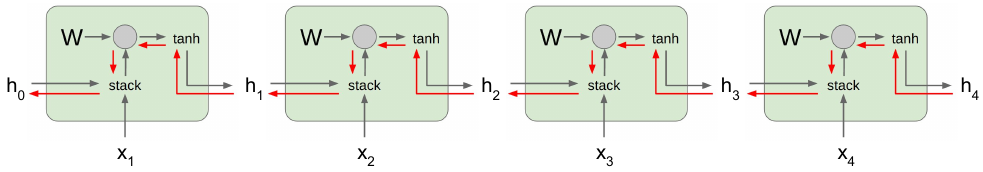
\includegraphics[width=12cm]{Figs/gradient_flow_rnn.png}
\caption{Vanilla RNN Gradient Flow, \href{https://kharshit.github.io/blog/2019/01/04/the-gradient-problem-in-rnn} 
        {Source}}

\end{figure}

\begin{itemize}
    \item RNN Training Issues
    \vspace{3mm}
    \begin{itemize}
        % \item Computing gradient of $h_0$ involves many factors of $W$ (and repeated 
        % $\mathbin{tanh}$)
        %     \\ What can we do to solve the problem? 
        % \vspace{3mm}
        \item \tc{keywords}{Exploding Gradients}
            \\ What can we do to solve exploding? 
        \item \tc{keywords}{Vanishing Gradients}
            \\ What can we do to solve vanishing?
        

    \end{itemize}
    

\end{itemize}
}
% %%%%%%%%%%%%%%%%%%%%%%%%%%%%%%%%%%%%%%%%%%%%%%%%%%%%%%%%%%%%%%%%%%%%%%%%
% \frame{\frametitle{Truncated Backpropagation Through Time (TBPTT)}
% \begin{figure}[!h]
% 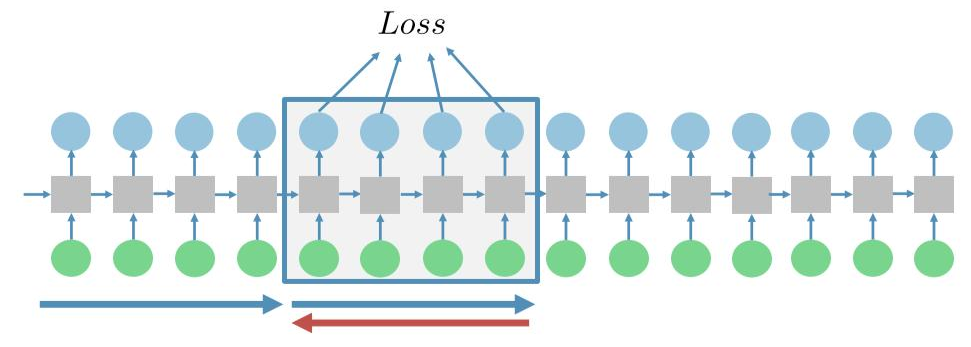
\includegraphics[width=8cm]{Figs/tbptt.png}
% \caption{TBPTT for $k_1 = k_2 = 4$, \href{https://www.programmersought.com/article/77613555017/} 
%         {Source}}

% \end{figure}


% \begin{itemize}
%     \item TBPTT Pseudo Code
%     \begin{enumerate}
%         \item for $t$ from $1$ to $T$ do
%         \item \hspace{1cm}Run the RNN one step
%         \item \hspace{1cm}if $t$ divides $k_1$ then
%         \item \hspace{1cm}\hspace{1cm}Run BPTT from $t$ down to $t - k_2$
%         \item \hspace{1cm}end if
%         \item end for 
%     \end{enumerate}


% \end{itemize}
% }
% %%%%%%%%%%%%%%%%%%%%%%%%%%%%%%%%%%%%%%%%%%%%%%%%%%%%%%%%%%%%%%%%%%%%%%%%
\section{LSTM-GRU}
%%%%%%%%%%%%%%%%%%%%%%%%%%%%%%%%%%%%%%%%%%
\frame{\frametitle{RNN Unit}
	
\begin{figure}[!h]
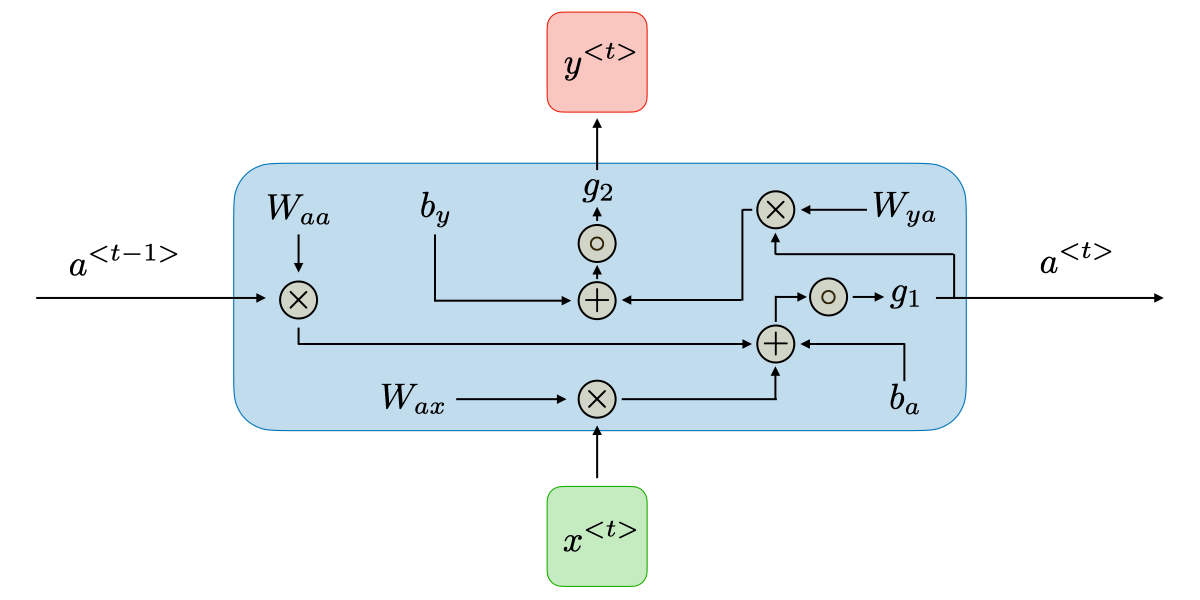
\includegraphics[width=8cm]{Figs/description-block-rnn-ltr.png}
\caption{RNN Unit, \href{https://stanford.edu/~shervine/teaching/cs-230/cheatsheet-recurrent-neural-networks} 
        {Source}}

\end{figure}


\begin{itemize}

	\item 
	For a simple RNN unit we had:

$$
a^{<t>} = g_1(W_{aa}a^{<t-1>} + W_{ax}x^{<t>}+b_a)
$$
$$
\centering y^{<t>} = g_2(W_{ga}a^{<t>}+b_y)
$$

\end{itemize}	

}

%%%%%%%%%%%%%%%%%%%%%%%%%%%%%%%%%%%%%%%%%%%%%%%%%%%%%%%%%%%%%%%%%%%%%%%%%%%%%%%%%%%%%%%%%%%%%%%
%%%%%%%%%%%%%%%%%%%%%%%%%%%%%%%%%%%%%%%%%%%%%%%%%%%%%%%%%%%%%%%%%%%%%%%%######
\frame{\frametitle{Gated Recurrent Unit (GRU)}
	
\begin{figure}[!h]
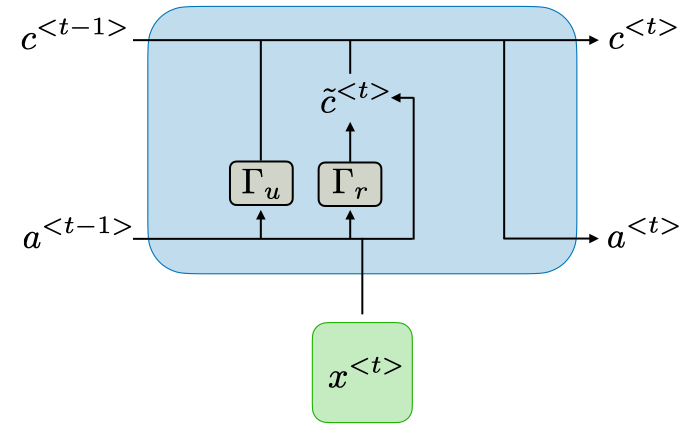
\includegraphics[width=5cm]{Figs/gru-ltr.png}
\caption{GRU Unit, \href{https://stanford.edu/~shervine/teaching/cs-230/cheatsheet-recurrent-neural-networks} 
        {Source}}
\centering
\end{figure}
$$
\Tilde{c}^{<t>} = \tanh(W_{c}[\Gamma_r * a^{<t-1>}, x^{<t>}]+ b_c)
$$
$$
\Gamma_r= \sigma(W_{r}[a^{<t-1>}, x^{<t>}]+b_r)
$$
$$
\Gamma_u= \sigma(W_{u}[a^{<t-1>}, x^{<t>}]+b_u)
$$
$$
c^{<t>} = \Gamma_u * \Tilde{c}^{<t>} + (1-\Gamma_u) * c^{<t-1>}
$$
$$
c^{<t>} = a^{<t>}
$$


}

%%%%%%%%%%%%%%%%%%%%%%%%%%%%%%%%%%%%%%%%%%%%%%%%%%%%%%%%%%%%%%%%%%%%%%%%%%%%%%%%%%%%%%%%%%%%%%%
%%%%%%%%%%%%%%%%%%%%%%%%%%%%%%%%%%%%%%%%%%%%%%%%%%%%%%%%%%%%%%%%%%%%%%%%######
\frame{\frametitle{Long Short-Term Memory (LSTM)}
	
\begin{figure}[!h]
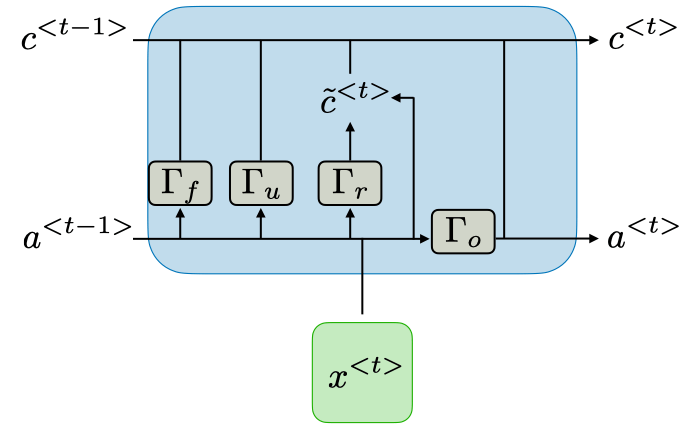
\includegraphics[width=4cm]{Figs/lstm-ltr.png}
\caption{LSTM Unit, \href{https://stanford.edu/~shervine/teaching/cs-230/cheatsheet-recurrent-neural-networks} 
        {Source}}
\end{figure}
$$
\Tilde{c}^{<t>} = \tanh(W_{c}[\Gamma_r * a^{<t-1>}, x^{<t>}]+ b_c)
$$
$$
\Gamma_r= \sigma(W_{r}[a^{<t-1>}, x^{<t>}]+b_r)
$$
$$
\Gamma_u= \sigma(W_{u}[a^{<t-1>}, x^{<t>}]+b_u)
$$
$$
\Gamma_o= \sigma(W_{o}[a^{<t-1>}, x^{<t>}]+b_o)
$$
$$
c^{<t>} = \Gamma_u * \Tilde{c}^{<t>} + (\Gamma_f) * c^{<t-1>}
$$
$$
a^{<t>} = \Gamma_o * c^{<t>}
$$


}

%%%%%%%%%%%%%%%%%%%%%%%%%%%%%%%%%%%%%%%%%%%%%%%%%%%%%%%%%%%%%%%%%%%%%%%%%%%%%%%%%%%%%%%%%%%%%%%
%%%%%%%%%%%%%%%%%%%%%%%%%%%%%%%%%%%%%%%%%%%%%%%%%%%%%%%%%%%%%%%%%%%%%%%%######
\frame{\frametitle{Type of Gates}
\vspace{-0.3cm}
\begin{figure}[!h]
\centering 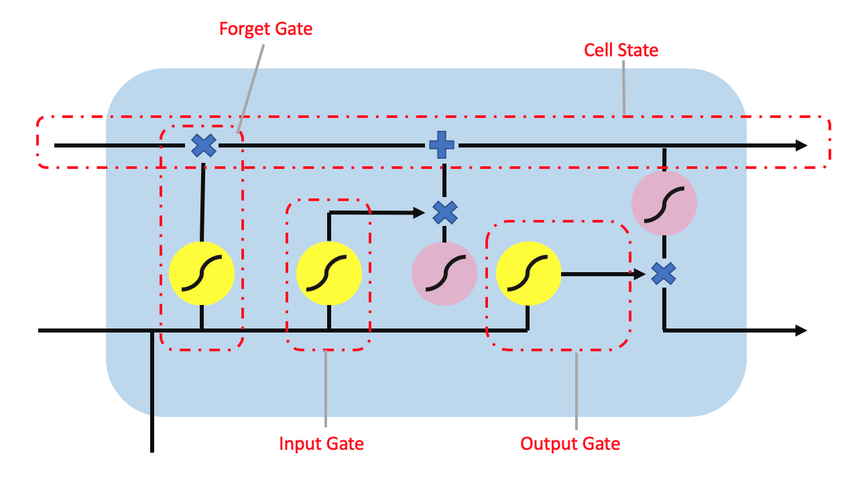
\includegraphics[width=6cm]{Figs/The-LSTM-unit-contain-a-forget-gate-output-gate-and-input-gate-The-yellow-circle.png}
\caption{Gates, \href{https://www.researchgate.net/figure/The-LSTM-unit-contain-a-forget-gate-output-gate-and-input-gate-The-yellow-circle_fig2_338717757}
        {Source}}
\end{figure}

\begin{itemize}

	\item Forget gate $\Gamma_f$: Erase a cell or not
\vspace{3mm}
	\item Relevance Gate $\Gamma_r$: Drop previous information
\vspace{3mm}
	\item Update Gate $\Gamma_u$: How much past should matter
\vspace{3mm} 
        \item Output gate $\Gamma_o$: How much to reveal of a cell

        
\end{itemize}	
	

}

%%%%%%%%%%%%%%%%%%%%%%%%%%%%%%%%%%%%%%%%%%%%%%%%%%%%%%%%%%%%%%%%%%%%%%%%%%%%%%%%%%%%%%%%%%%%%%%
%%%%%%%%%%%%%%%%%%%%%%%%%%%%%%%%%%%%%%%%%%%%%%%%%%%%%%%%%%%%%%%%%%%%%%%%######
\frame{\frametitle{LSTM Walk Through}
\begin{itemize}
    \item The first step in our LSTM is to decide what information we’re going to throw away from the cell state.
\end{itemize}
\begin{figure}[!h]
\centering 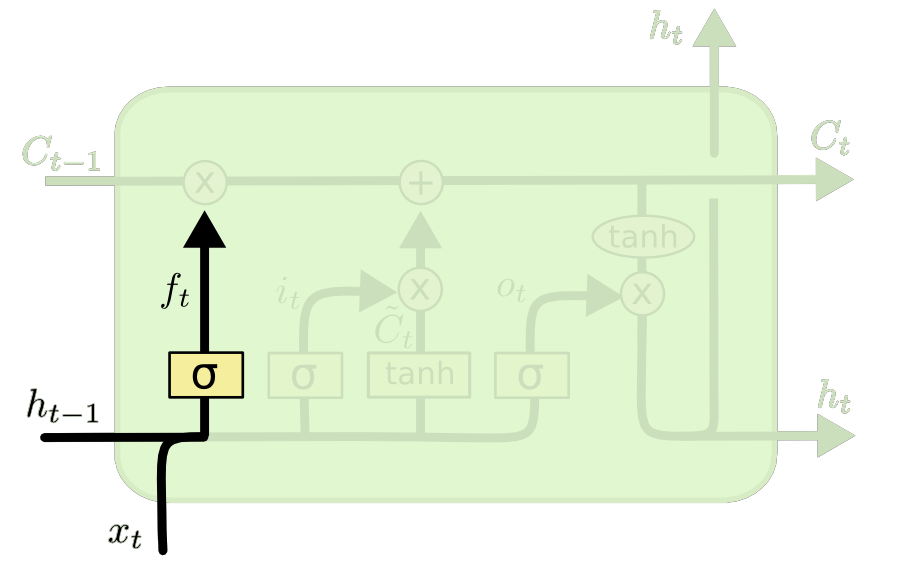
\includegraphics[width=6cm]{Figs/LSTM3-focus-f.png}
\caption{Forget Gate Layer, \href{https://colah.github.io/posts/2015-08-Understanding-LSTMs/}
        {Source}}
\end{figure}
	

}

%%%%%%%%%%%%%%%%%%%%%%%%%%%%%%%%%%%%%%%%%%%%%%%%%%%%%%%%%%%%%%%%%%%%%%%%%%%%%%%%%%%%%%%%%%%%%%%
%%%%%%%%%%%%%%%%%%%%%%%%%%%%%%%%%%%%%%%%%%%%%%%%%%%%%%%%%%%%%%%%%%%%%%%%######
\frame{\frametitle{LSTM Walk Through}
\begin{itemize}
    \item The next step is to decide what new information we’re going to store in the cell state.
\end{itemize}
\begin{figure}[!h]
\centering 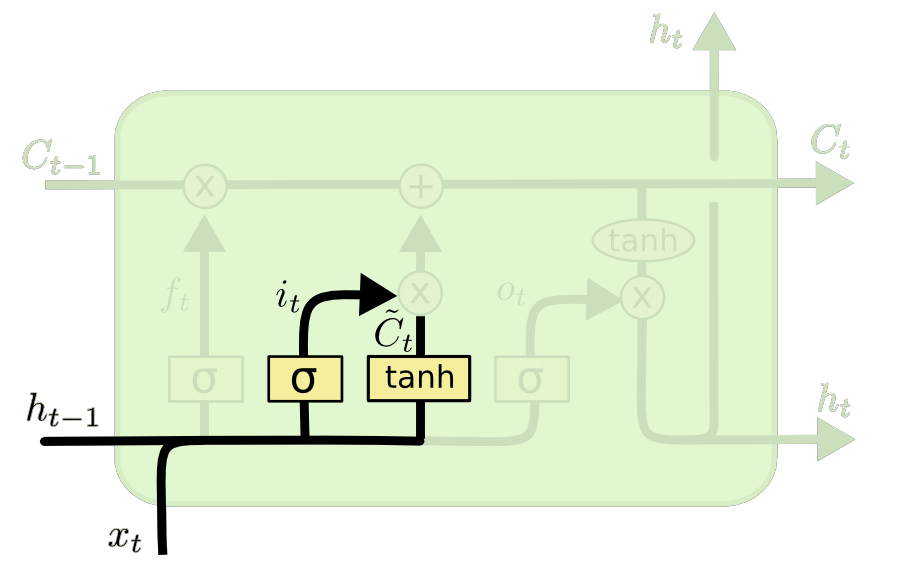
\includegraphics[width=6cm]{Figs/LSTM3-focus-i.png}
\caption{Input Gate Layer, \href{https://colah.github.io/posts/2015-08-Understanding-LSTMs/}
        {Source}}
\end{figure}	

	

}

%%%%%%%%%%%%%%%%%%%%%%%%%%%%%%%%%%%%%%%%%%%%%%%%%%%%%%%%%%%%%%%%%%%%%%%%%%%%%%%%%%%%%%%%%%%%%%%
%%%%%%%%%%%%%%%%%%%%%%%%%%%%%%%%%%%%%%%%%%%%%%%%%%%%%%%%%%%%%%%%%%%%%%%%######
\frame{\frametitle{LSTM Walk Through}
\begin{itemize}
    \item It’s now time to update the old cell state, Ct−1, into the new cell state Ct.
\end{itemize}
\begin{figure}[!h]
\centering 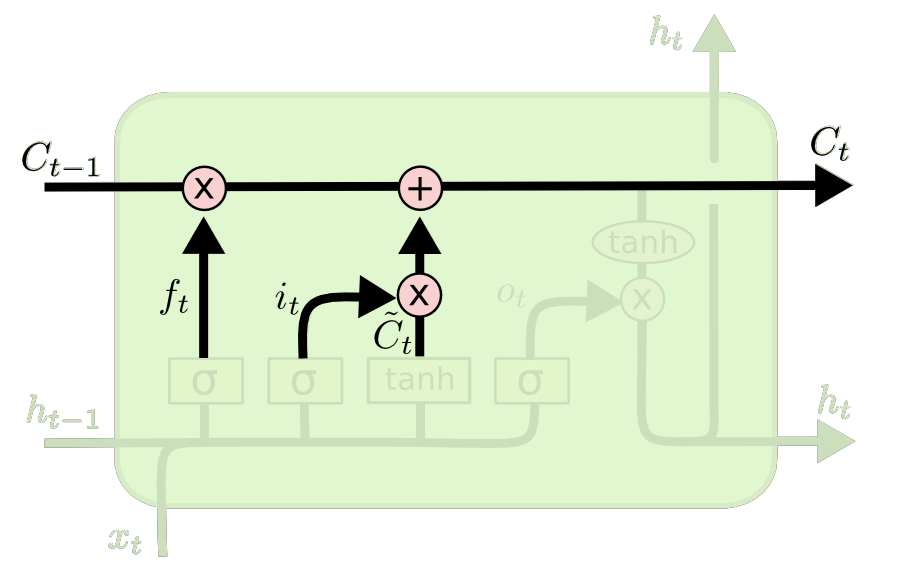
\includegraphics[width=6cm]{Figs/LSTM3-focus-C.png}
\caption{Update Cell State, \href{https://colah.github.io/posts/2015-08-Understanding-LSTMs/}
        {Source}}
\end{figure}	

}

%%%%%%%%%%%%%%%%%%%%%%%%%%%%%%%%%%%%%%%%%%%%%%%%%%%%%%%%%%%%%%%%%%%%%%%%%%%%%%%%%%%%%%%%%%%%%%%
%%%%%%%%%%%%%%%%%%%%%%%%%%%%%%%%%%%%%%%%%%%%%%%%%%%%%%%%%%%%%%%%%%%%%%%%######
\frame{\frametitle{LSTM Walk Through}
\begin{itemize}
    \item Finally, we need to decide what we’re going to output. This output will be based on our cell state
\end{itemize}
\begin{figure}[!h]
\centering 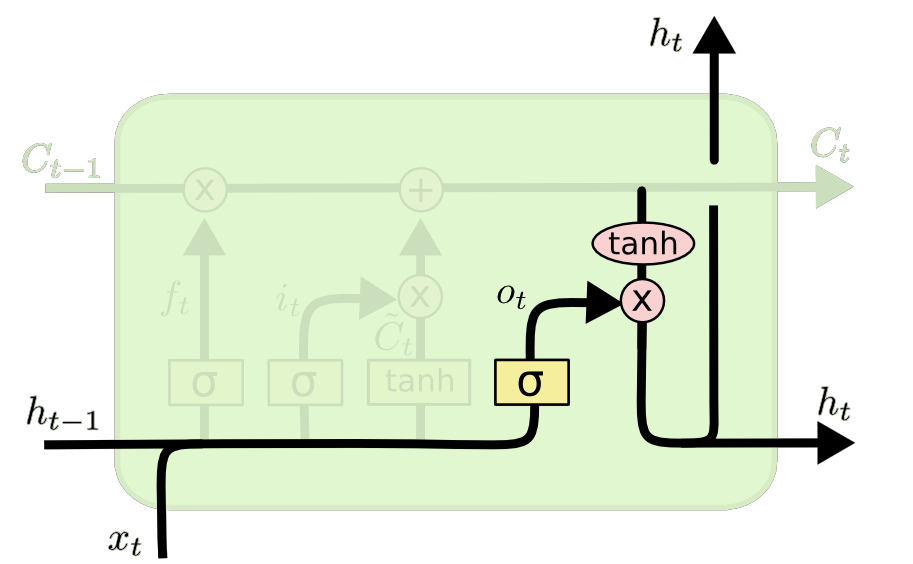
\includegraphics[width=6cm]{Figs/LSTM3-focus-o.png}
\caption{Output Gate Layer, \href{https://colah.github.io/posts/2015-08-Understanding-LSTMs/}
        {Source}}
\end{figure}	

}

%%%%%%%%%%%%%%%%%%%%%%%%%%%%%%%%%%%%%%%%%%%%%%%%%%%%%%%%%%%%%%%%%%%%%%%%%%%%%%%%%%%%%%%%%%%%%%%
%%%%%%%%%%%%%%%%%%%%%%%%%%%%%%%%%%%%%%%%%%%%%%%%%%%%%%%%%%%%%%%%%%%%%%%%######
\frame{\frametitle{Why LSTMs?}

\vspace{-2cm}
\begin{itemize}
	\item The LSTM does have the ability to remove and add information to the cell state.
\vspace{3mm}

	\item The gates in the previous slide let the information to pass through the units.
 
\vspace{3mm}
	\item The gates value are between zero and one and specify \tc{keywords}{how much information should be let through}.
\vspace{3mm}
        \item They also somehow solve the \tc{keywords}{vanishing gradient}.
        \vspace{3mm}
        
        \item We can use more blocks of them so there will be more information to remember.
        
\end{itemize}	
	

}

%%%%%%%
%%%%%%%%%%%%%%%%%%%%%%%%%%%%%%%%%%%%%%%%%%%%%%%%%%%%%%%%%%%%%%%%%%%%%%%%######
\frame{\frametitle{How LSTMs solve vanishing gradients}
\begin{figure}[!h]
\centering 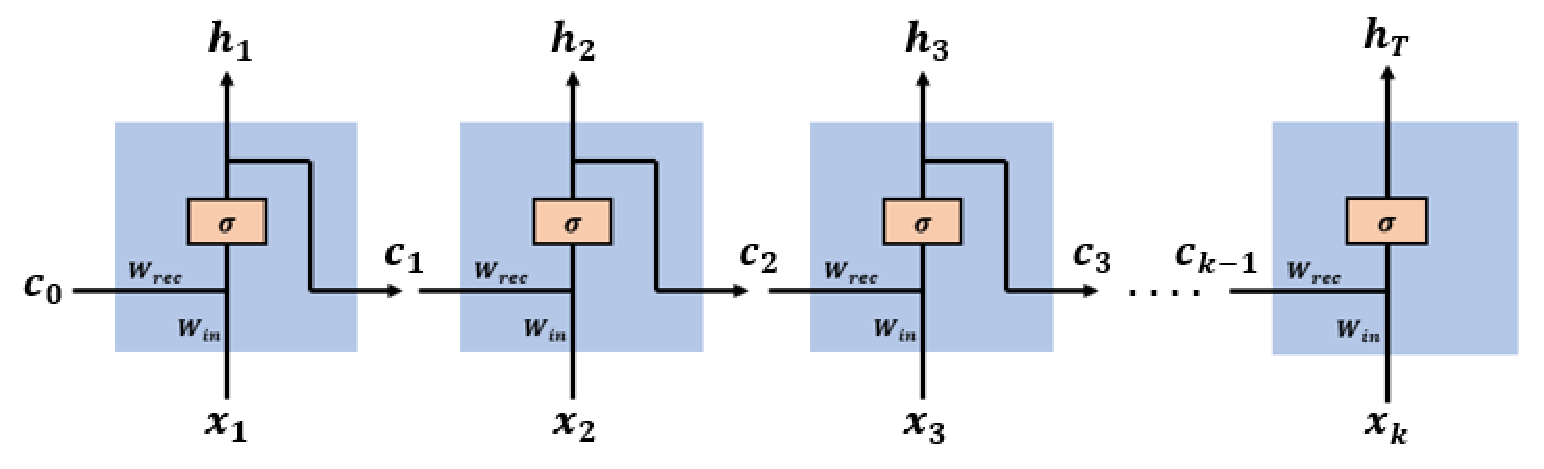
\includegraphics[width=10cm]{Figs/rnn-bp.eps}
\caption{Simple Recurrent Neural Network, \href{https://medium.datadriveninvestor.com/how-do-lstm-networks-solve-the-problem-of-vanishing-gradients-a6784971a577}
        {Source}}
\end{figure}

	

}

%%%%%%%%%%%%%%%%%%%%%%%%%%%%%%%%%%%%%%%%%%%%%%%%%%%%%%%%%%%%%%%%%%%%%%%%%%%%%%%%%%%%%%%%%%%%%%%
%%%%%%%%%%%%%%%%%%%%%%%%%%%%%%%%%%%%%%%%%%%%%%%%%%%%%%%%%%%%%%%%%%%%%%%%######
\frame{\frametitle{How LSTMs solve vanishing gradients}
\begin{itemize}
\item In Vanilla RNN we have
$$
\frac{\partial L}{\partial W} = \sum_{t=1}^{T} \frac{\partial L_t}{\partial W}
$$
\begin{align*}
\frac{\partial L_k}{\partial W} = \frac{\partial L_k}{\partial h_k} \frac{\partial h_k}{\partial c_k} \dots \frac{\partial c_2}{\partial c_1} \frac{\partial c_1}{\partial W} 
 = \frac{\partial L_k}{\partial h_k} \frac{\partial h_k}{\partial c_k} (\prod_{t=2}^{k} \frac{\partial c_t}{\partial c_{t-1}}) \frac{\partial c_1}{\partial W}
\end{align*}

$$
\frac{\partial c_t}{\partial c_{t-1}} = \sigma'(W_{rec}.c_{t-1} + W_{in}.x_t)W_{rec}
$$

\begin{align*}
\frac{\partial L_k}{\partial W} = \frac{\partial L_k}{\partial h_k} \frac{\partial h_k}{\partial c_k} (\prod_{t=2}^{k} \sigma'(W_{rec}.c_{t-1} + W_{in}.x_t)W_{rec}) \frac{\partial c_1}{\partial W}
\end{align*}


\item For large K the gradient tends to vanish or if $W_{rec}$ is large enough it cause exploding gradient which is solved by \textit{Gradient Clipping}.
\end{itemize}

	

}
%%%%%%%
%%%%%%%%%%%%%%%%%%%%%%%%%%%%%%%%%%%%%%%%%%%%%%%%%%%%%%%%%%%%%%%%%%%%%%%%######

\frame{\frametitle{How LSTMs solve vanishing gradients}
\begin{figure}[!h]
\centering 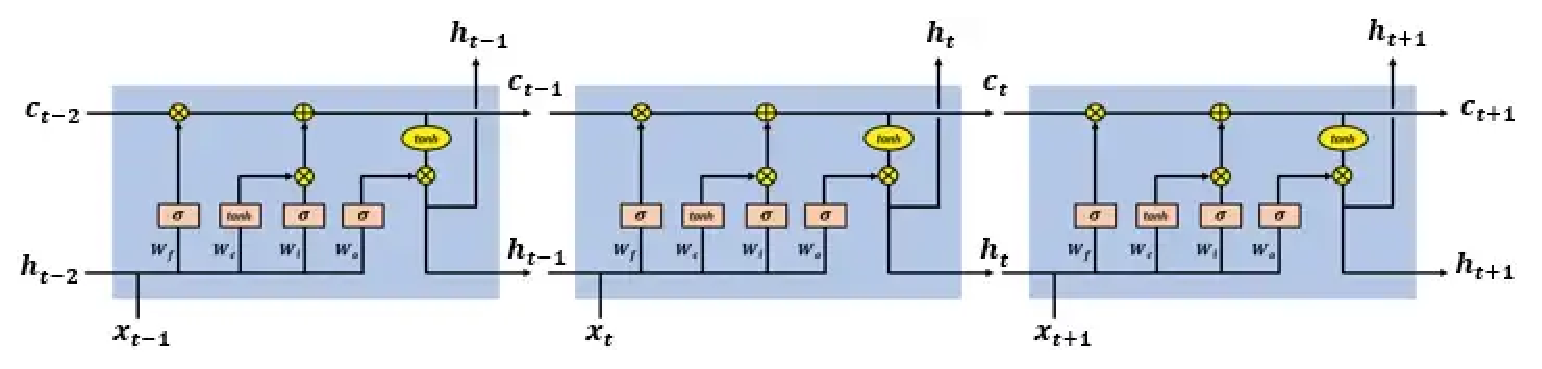
\includegraphics[width=10cm]{Figs/lstm-bp.eps}
\caption{LSTM Network, \href{https://medium.datadriveninvestor.com/how-do-lstm-networks-solve-the-problem-of-vanishing-gradients-a6784971a577}
        {Source}}
\end{figure}

	

}

%%%%%%%%%%%%%%%%%%%%%%%%%%%%%%%%%%%%%%%%%%%%%%%%%%%%%%%%%%%%%%%%%%%%%%%%%%%%%%%%%%%%%%%%%%%%%%%
%%%%%%%%%%%%%%%%%%%%%%%%%%%%%%%%%%%%%%%%%%%%%%%%%%%%%%%%%%%%%%%%%%%%%%%%######
\frame{\frametitle{How LSTMs solve vanishing gradients}
\begin{itemize}
\item In LSTM we also have

\begin{align*}
\frac{\partial L_k}{\partial W} =  \frac{\partial L_k}{\partial h_k} \frac{\partial h_k}{\partial c_k} (\prod_{t=2}^{k} \frac{\partial c_t}{\partial c_{t-1}}) \frac{\partial c_1}{\partial W}
\end{align*}
\item But 
$$
c^{t} = \Gamma_u * \Tilde{c}^{t} + (\Gamma_f) * c^{t-1}
$$
$$
\frac{\partial c_t}{\partial c_{t-1}} = \frac{\partial \Gamma_f}{\partial c_{t-1}}.c_{t-1} + \Gamma_f + \frac{\partial \Gamma_u}{\partial c_{t-1}}.\Tilde{c_{t}} + \frac{\partial \Tilde{c_t}}{\partial c_{t-1}}.\Gamma_u
$$

\item Consider that the \textit{forget gate} is added to other terms and allows better control of gradient values. But it doesn't guarantee that there is no vanishing or exploding in gradient.
\end{itemize}



}

%%%%%%%%%%%%%%%%%%%%%%%%%%%%%%%%%%%%%%%%%%%%%%%%%%%%%%%%%%%%%%%%%%%%%%%%%%%%%%%%%%%%%%%%%%%%%%%
\section{Bidirectional RNN}
%%%%%%%%%%%%%%%%%%%%%%%%%%%%%%%%%%%%%%%%%%%%%%%%%%%%%%%%%%%%%%%%%%%%%%%%######
\frame{\frametitle{Bidirectional RNN}
\begin{itemize}
\item How to get information from future?
\end{itemize}
\begin{figure}[!h]
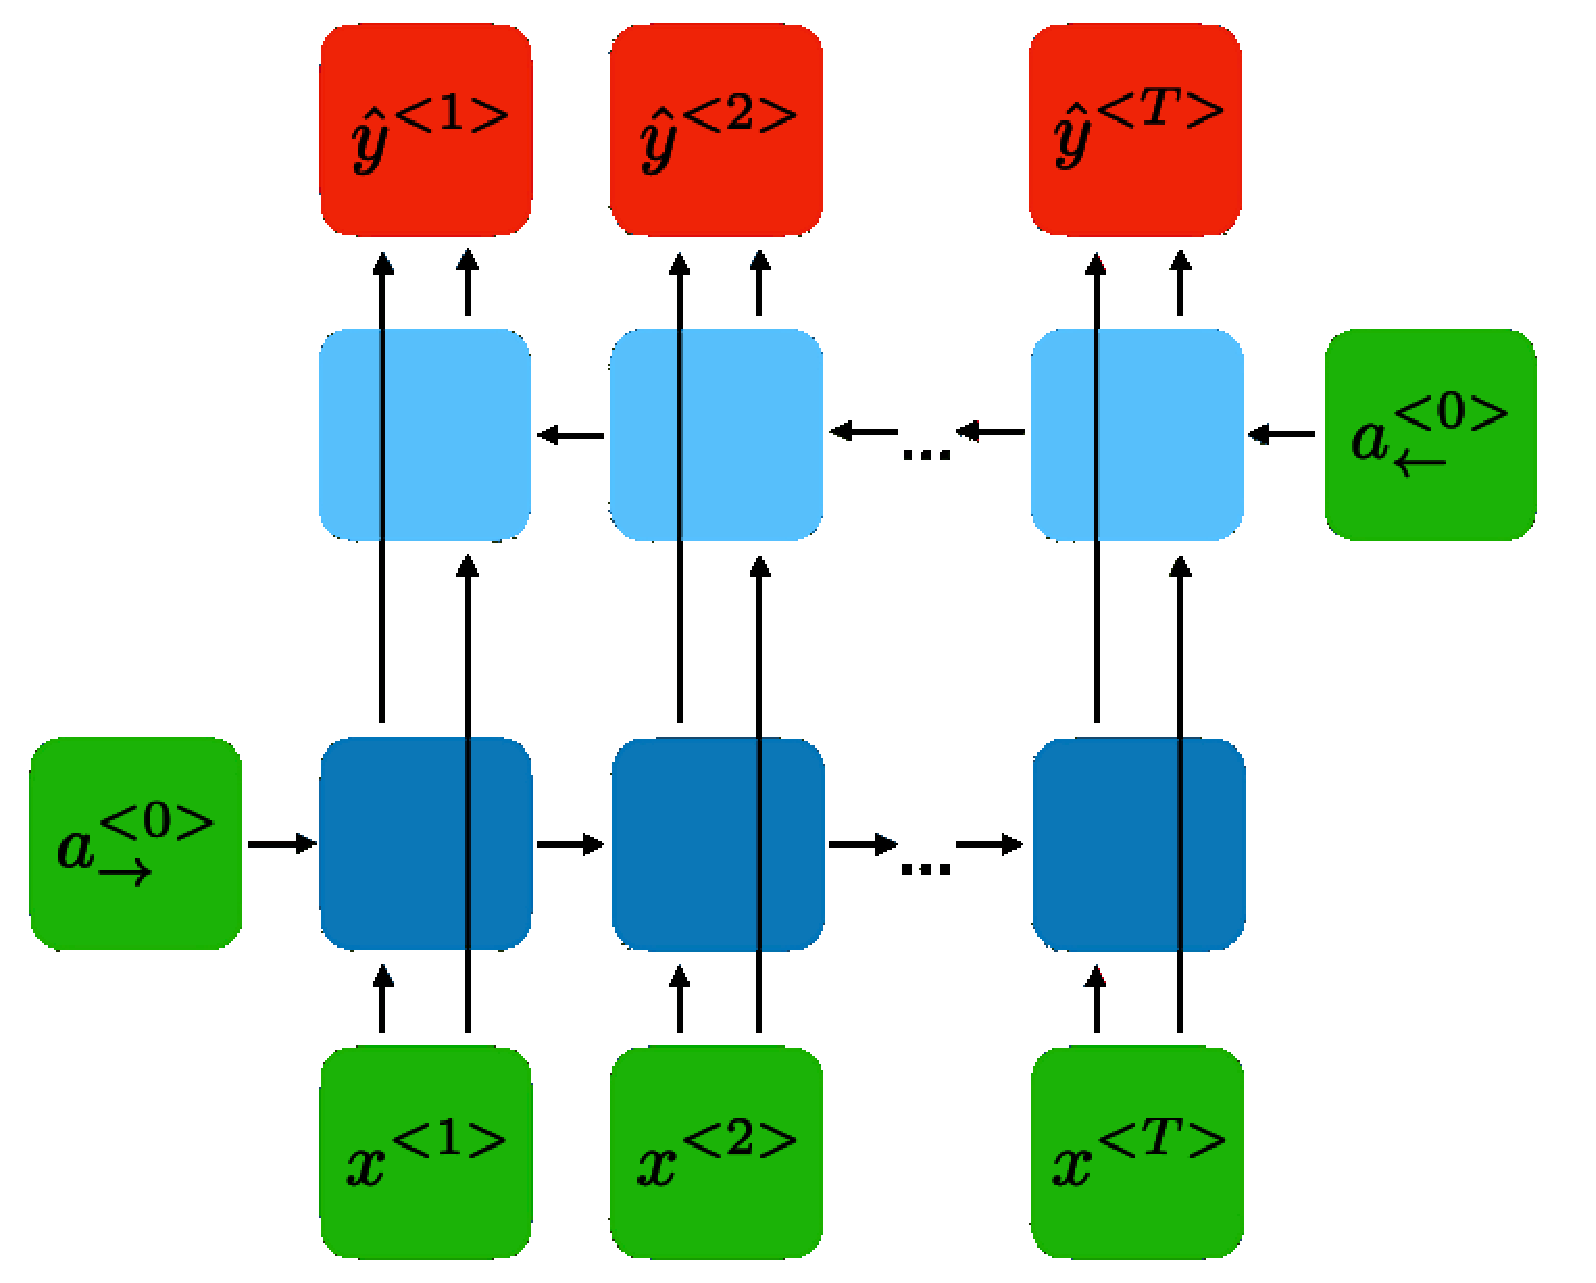
\includegraphics[width=5cm]{Figs/bidirectional-rnn-ltr.eps}
\caption{BRNN, \href{https://stanford.edu/~shervine/teaching/cs-230/cheatsheet-recurrent-neural-networks} 
        {Source}}
\centering
\end{figure}

$$
y^{<t>} = g(W_y[\vec{a}^{<t>}, \cev{a}^{<T-t>}] + b_y)
$$


}

%%%%%%%%%%%%%%%%%%%%%%%%%%%%%%%%%%%%%%%%%%%%%%%%%%%%%%%%%%%%%%%%%%%%%%%%%%%%%%%%%%%%%%%%%%%%%%%
%%%%%%%%%%%%%%%%%%%%%%%%%%%%%%%%%%%%%%%%%%%%%%%%%%%%%%%%%%%%%%%%%%%%%%%%######
\frame{\frametitle{Bidirectional RNN}
\vspace{-1cm}
\begin{itemize}
    \item They are usually used in natural language processing.

\vspace{3mm}
    
    \item They are powerful for modeling dependencies between words and phrases in both directions of the sequence because every component of an input sequence has information from both the past and present.

\end{itemize}
\begin{figure}[!h]
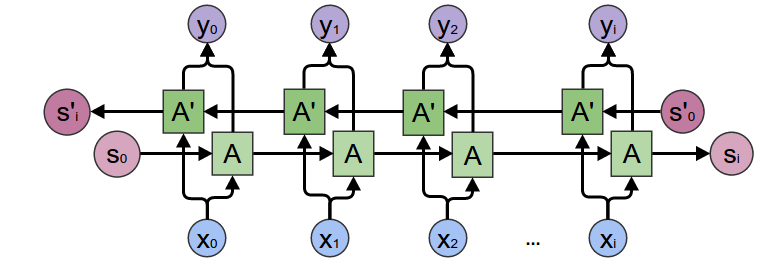
\includegraphics[width=8cm]{Figs/bidir.png}
\caption{BRNN, \href{http://colah.github.io/posts/2015-09-NN-Types-FP/} 
        {Source}}
\centering
\end{figure}

}

%%%%%%%%%%%%%%%%%%%%%%%%%%%%%%%%%%%%%%%%%%%%%%%%%%%%%%%%%%%%%%%%%%%%%%%%%%%%%%%%%%%%%%%%%%%%%%%
%%%%%%%%%%%%%%%%%%%%%%%%%%%%%%%%%%%%%%%%%%%%%%%%%%%%%%%%%%%%%%%%%%%%%%%%######
\frame{\frametitle{Back-propagation in BRNN}
\begin{itemize}
\item It is exactly the same as simple RNN
\end{itemize}
\begin{figure}[!h]
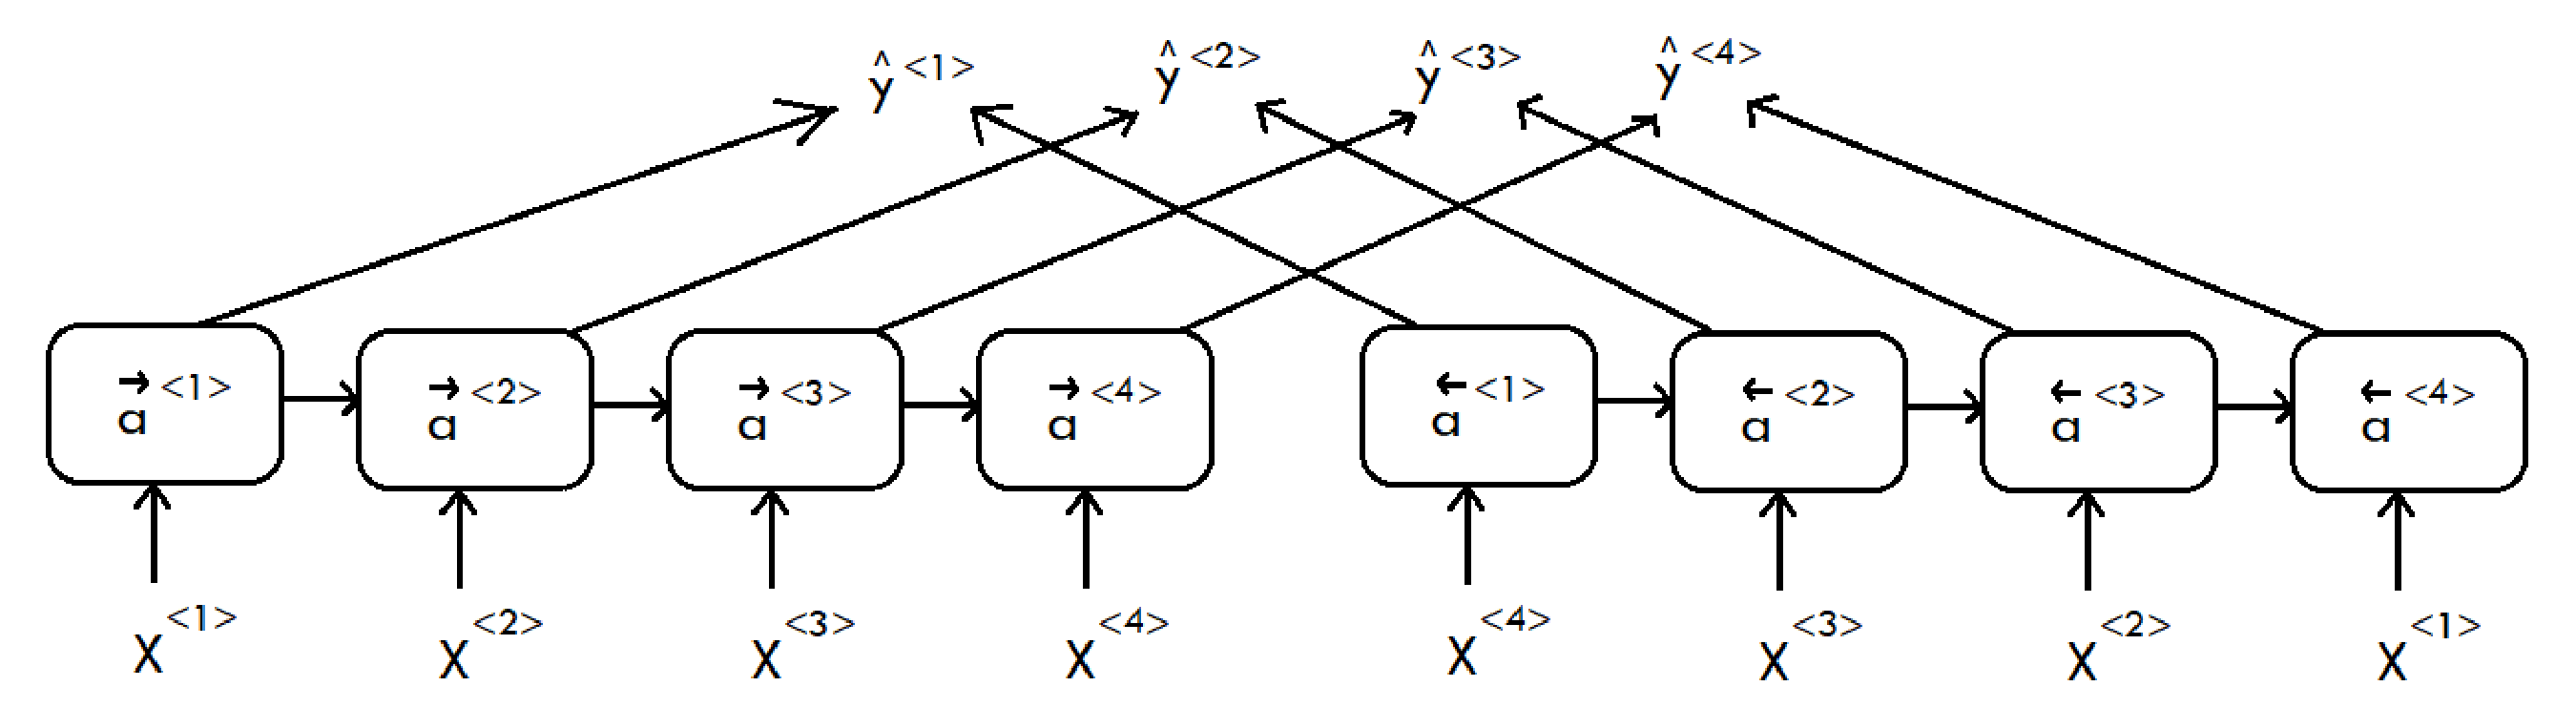
\includegraphics[width=10cm]{Figs/bpbbrn.eps}
\caption{BRNN, \href{https://ai.stackexchange.com/questions/24013/how-does-back-propagation-through-time-work-for-optimizing-the-weights-of-a-bidi} 
        {Source}}
\centering
\end{figure}

}
%%%%%%%%%%%%%%%%%%%%%%%%%%%%%%%%%%%%%%%%%%%%%%%%%%%%%%%%%%%%%%%%%%%%%%%%%%%%%%%%%%%%%
\section{Encoder-Decoder}
%%%%%
\frame{\frametitle{Encoder-Decoder}

\begin{itemize}
\item If we want an output with a \tc{keywords}{different length} from the
input (e.g. Machine Translation), what should we do?
\vspace{3mm}
\item Which \tc{keywords}{alignment} method should we use?
\end{itemize}

\begin{figure}[!h]
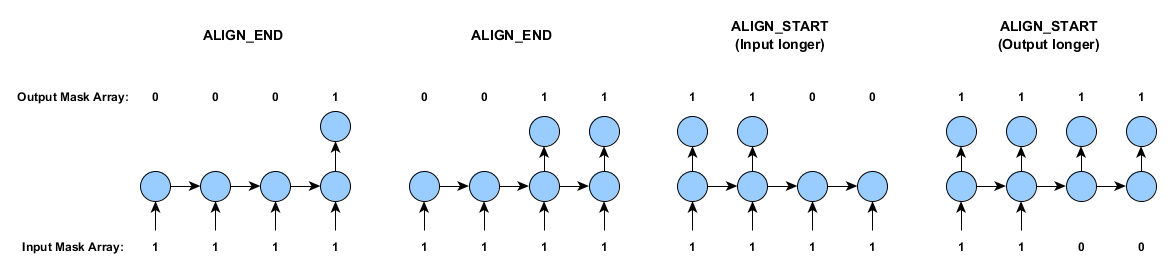
\includegraphics[width=12cm]{Figs/rnn_seq_alignment.png}
\caption{Problems in Sequence-to-Sequence Models, \href{https://mgubaidullin.github.io/deeplearning4j-docs/usingrnns.html} 
        {Source}}
\end{figure}

}
%%%%%%%%%%%%%%%%%%%%%%%%%%%%%%%%%%%%%%%%%%%%%%%%%%%%%%%%%%%%%%%%%%%%%%%%%%%%%%%%%%%%%
%%%%%
\frame{\frametitle{Encoder-Decoder}
\begin{center}
    Encoder-Decoder architecture could be a solution.
\end{center}

\begin{figure}[!h]
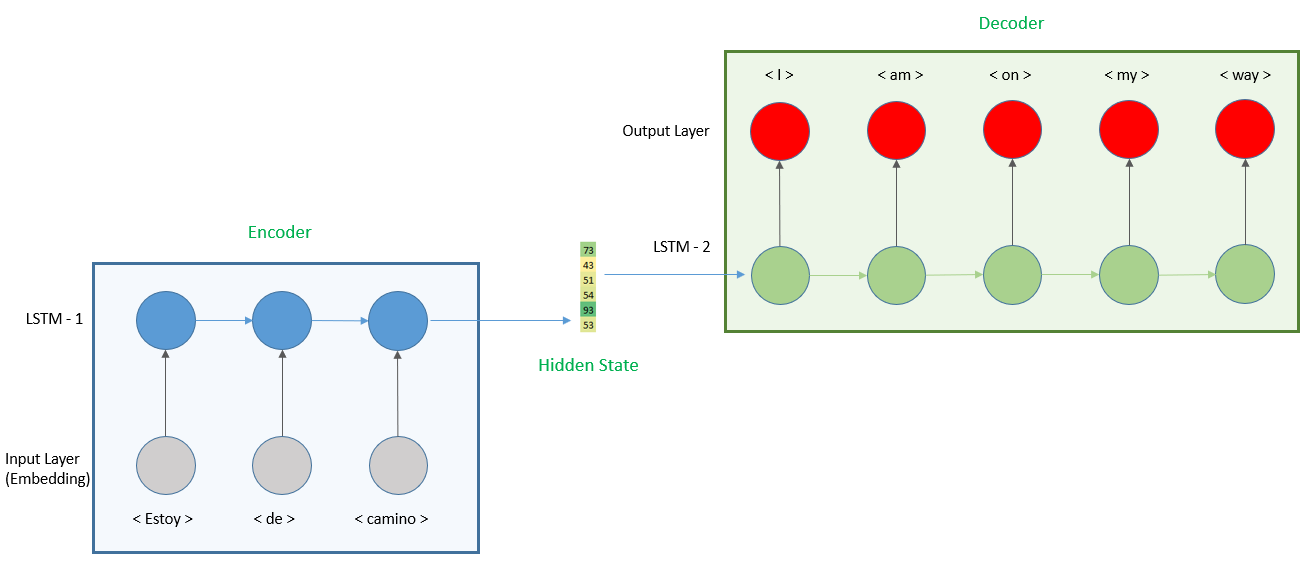
\includegraphics[width=12cm]{Figs/encdec2.png}
\caption{Encoder-Decoder, \href{https://towardsdatascience.com/how-to-build-an-encoder-decoder-translation-model-using-lstm-with-python-and-keras-a31e9d864b9b} 
        {Source}}
\end{figure}

}
%%%%%%%%%%%%%%%%%%%%%%%%%%%%%%%%%%%%%%%%%%%%%%%%%%%%%%%%%%%%%%%%%%%%%%%%%%%%%%%%%%%%%
\frame{\frametitle{Encoder-Decoder}
\vspace{-1cm}
\begin{figure}[!h]
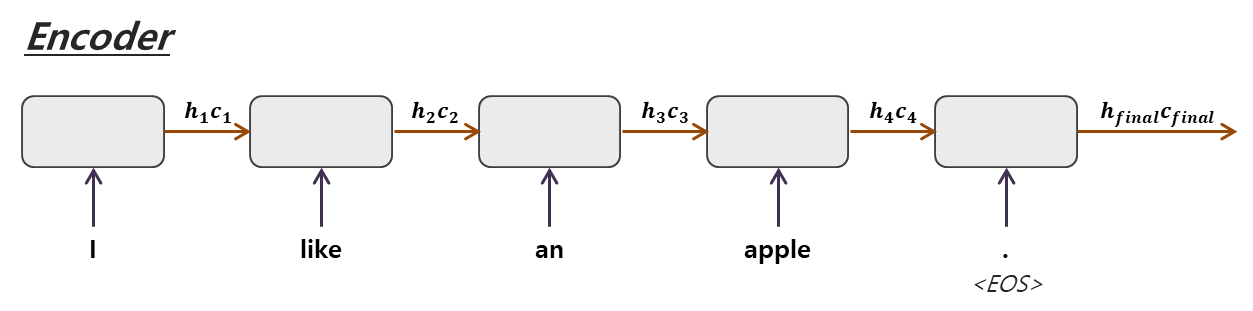
\includegraphics[width=10cm]{Figs/encoder.png}
\caption{Encoder, \href{https://yjjo.tistory.com/35} 
        {Source}}
\end{figure}

\begin{itemize}
        \item \textbf{Encoder:} The encoder processes the input sequence and compresses the information into a fixed length vector, known as the context vector. 
\end{itemize}

}
%%%%%%%%%%%%%%%%%%%%%%%%%%%%%%%%%%%%%%%%%%%%%%%%%%%%%%%%%%%%%%%%%%%%%%%%%%%%%%%%%%%%%
\frame{\frametitle{Encoder-Decoder}

\begin{figure}[!h]
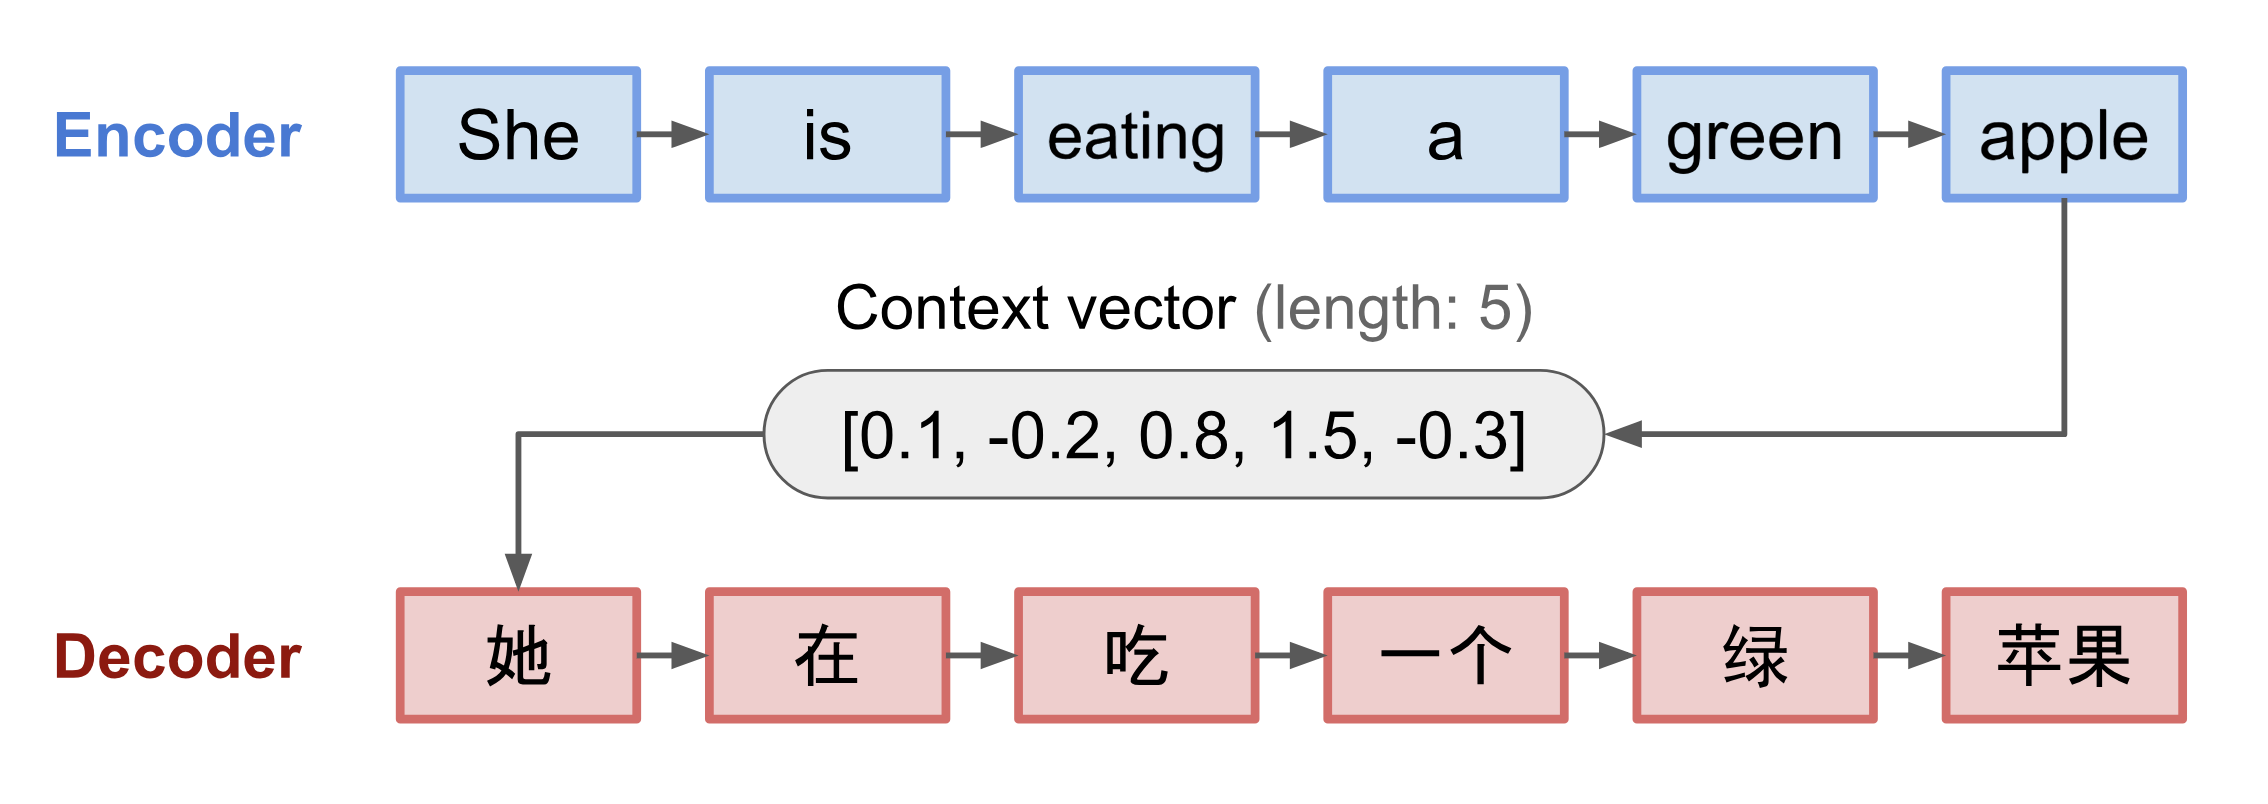
\includegraphics[width=8cm]{Figs/encoder-decoder-example.png}
\caption{Context Vector, \href{https://lilianweng.github.io/posts/2018-06-24-attention/} 
        {Source}}
\end{figure}

\begin{itemize}
        \item \textbf{Context Vector (Hidden State):} This vector is expected to convey the meaning of the whole source sequence from the encoder to the decoder.
     \begin{itemize}
         \item The early work considered the last state of the encoder network as the context vector.
     \end{itemize}

\end{itemize}

}
%%%%%%%%%%%%%%%%%%%%%%%%%%%%%%%%%%%%%%%%%%%%%%%%%%%%%%%%%%%%%%%%%%%%%%%%%%%%%%%%%%%%%
\frame{\frametitle{Encoder-Decoder}

\begin{figure}[!h]
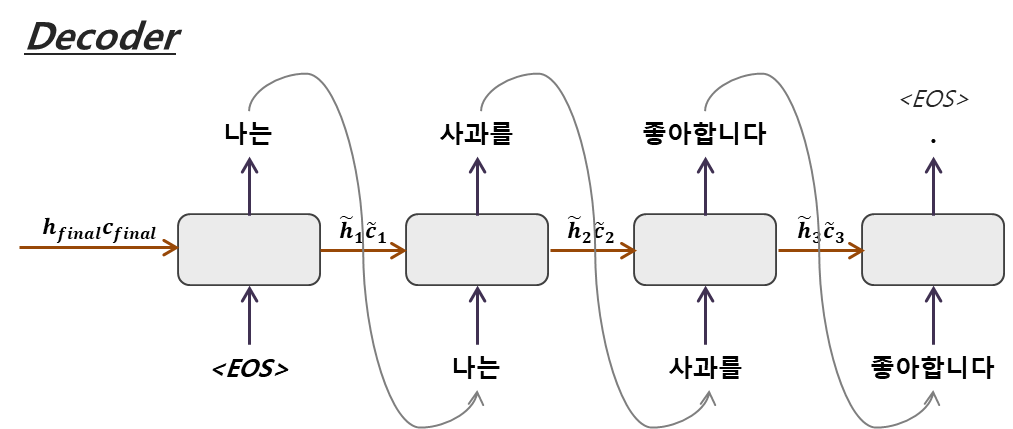
\includegraphics[width=8cm]{Figs/decoder.png}
\caption{Decoder, \href{https://yjjo.tistory.com/35} 
        {Source}}
\end{figure}

\begin{itemize}
        \item \textbf{Decoder:} The decoder uses the context vector to output the desired target sequence.
\end{itemize}
}
%%%%%%%%%%%%%%%%%%%%%%%%%%%%%%%%%%%%%%%%%%%%%%%%%%%%%%%%%%%%%%%%%%%%%%%%%%%%%%%%%%%%%
\frame{\frametitle{Encoder-Decoder Limitations}
\vspace{-1cm}
\begin{figure}[!h]
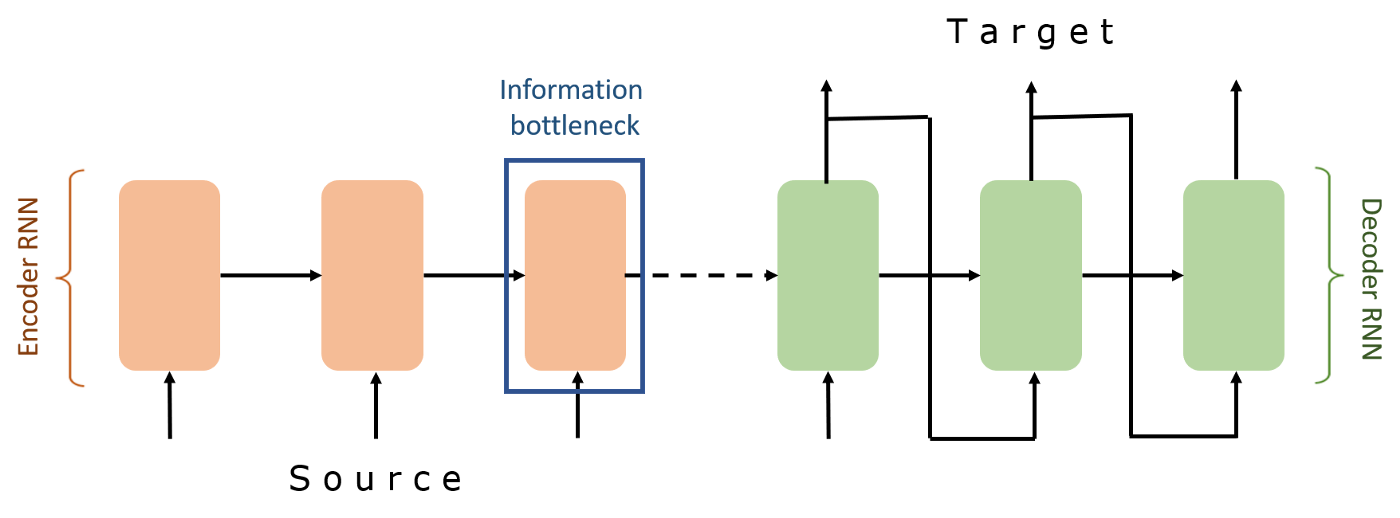
\includegraphics[width=8cm]{Figs/bottleneck.png}
        \caption{Bottleneck Phenomenon, \href{https://towardsdatascience.com/attention-and-its-different-forms-7fc3674d14dc} 
        {Source}}
\end{figure}

\begin{itemize}
        \item The context vector is \tc{keywords}{bottleneck}. 
        By increasing the length of the input sequence, the model captures the essential information roughly. How to solve it?
\end{itemize}

}
%%%%%%%%%%%%%%%%%%%%%%%%%%%%%%%%%%%%%%%%%%%%%%%%%%%%%%%%%%%%%%%%%%%%%%%%%%%%%%%%%%%%%
\frame{\frametitle{Encoder-Decoder Limitations}


\begin{figure}[!h]
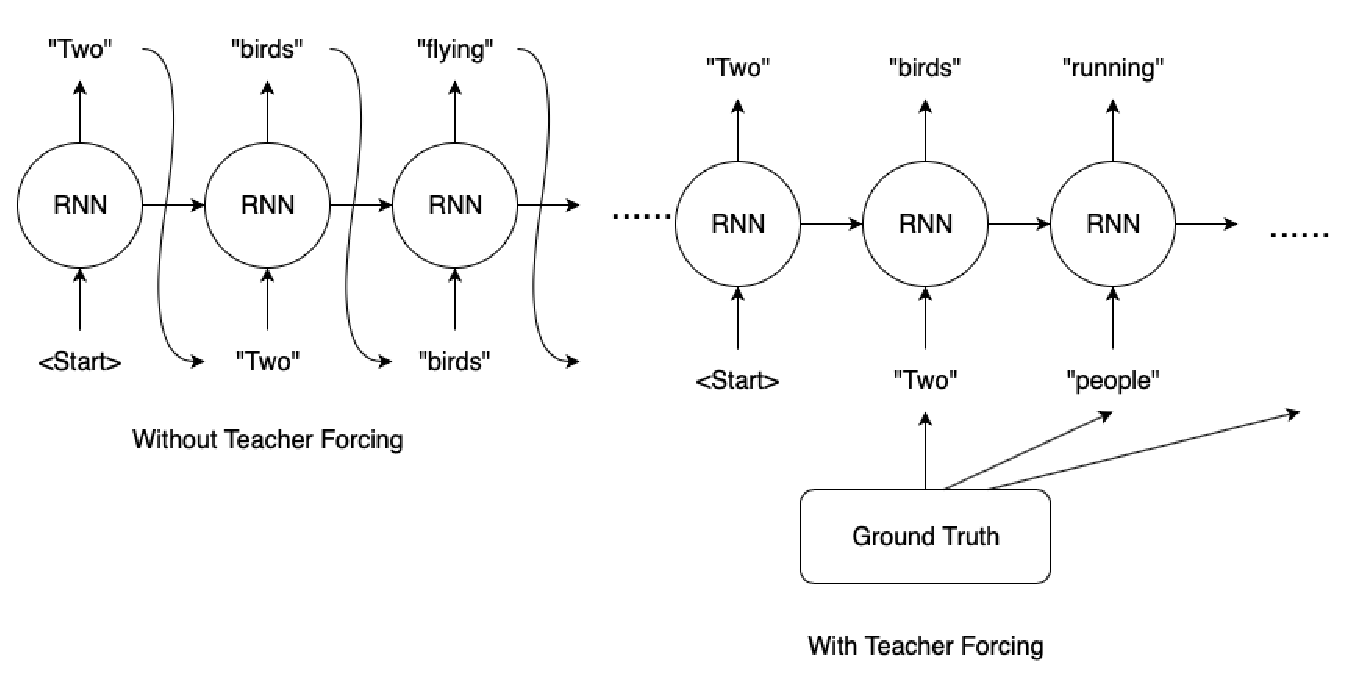
\includegraphics[width=10cm]{Figs/tf_ende.eps}
        \caption{Teacher Forcing in Decoder Side, \href{https://towardsdatascience.com/what-is-teacher-forcing-3da6217fed1c} 
        {Source}}
\end{figure}

}
%%%%%
\section{Teacher Forcing}
%%%%%%%%%%%%%%%%%%%%%%%%%%%%%%%%%%%%%%%%%%%%%%%%%%%%%%%%%%%%%%%%%%%%%%%%######
\frame{\frametitle{Teacher Forcing}

\begin{itemize}

\item Teacher forcing is a method for training recurrent neural networks more efficiently.
\vspace{3mm}
\item Teacher forcing works by using the actual output at the current time step $y^{(t-1)}$ as input in the next time step, rather than the $o^{(t-1)}$generated by the network.

\end{itemize}
\begin{figure}[!h]
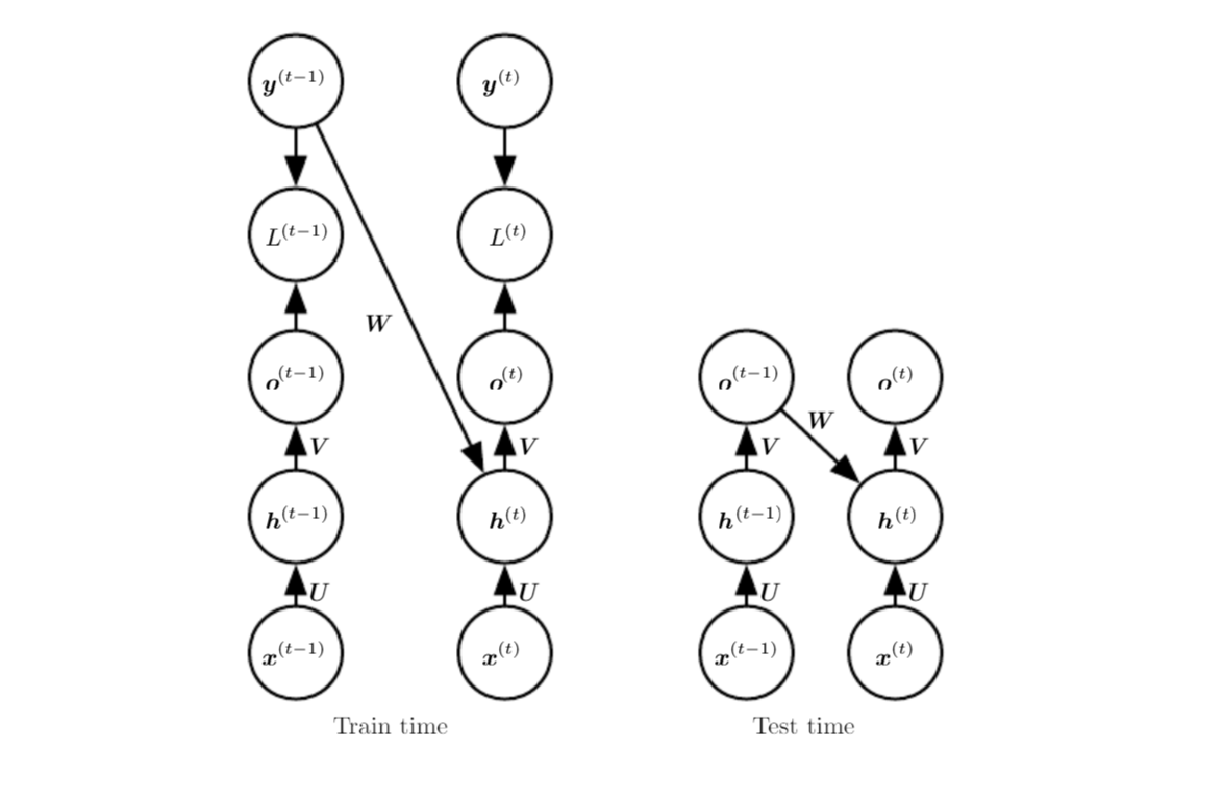
\includegraphics[width=8cm]{Figs/fig10-6.eps}
\caption{Teacher Forcing, \href{https://www.arashash.com/2020-02-23-deeplearning-ch10-lect2/} 
        {Source}}
\centering
\end{figure}

}
%%%%%%%%%%%%%%%%%%%%%%%%%%%%%%%%%%%%%%%%%%%%%%%%%%%%%%%%%%%%%%%%%%%%%%%%%%%%%%%%%%%%%%%%%%%%%%%
%%%%%%%%%%%%%%%%%%%%%%%%%%%%%%%%%%%%%%%%%%%%%%%%%%%%%%%%%%%%%%%%%%%%%%%%######
\frame{\frametitle{Teacher Forcing}

\vspace{-1cm}
\begin{itemize}

\item  At the early stages of training, the predictions of the model are very bad.
\vspace{5mm}
\item If we do not use Teacher Forcing, the hidden states of the model will be updated by a sequence of wrong predictions, \tc{keywords} {errors will accumulate.}
\vspace{5mm}
\item It will be difficult for the model to learn from that.
\vspace{5mm}

\item This technique allows us to prevent backpropagation through time which was complex and time-consuming. With teacher forcing the model will be \tc{keywords} {trained faster}.


\end{itemize}

}
%%%%%%%%%%%%%%%%%%%%%%%%%%%%%%%%%%%%%%%%%%%%%%%%%%%%%%%%%%%%%%%%%%%%%%%%%%%%%%%%%%%%%
\section{Beam Search}
%%%%%%%%%%%%%%%%%%%%%%%%%%%%%%%%%%%%%%%%%%%%%%%%%%%%%%%%%%%%%%%%%%%%%%%%%%%%%%%%%%%%%
\frame{\frametitle{Search Strategy}
\begin{figure}[!h]
\includegraphics[width=8cm]{Figs/machine_translation.eps}
        \caption{Simple Machine Translation Model, \href{https://www.guru99.com/seq2seq-model.html} 
        {Source}}
\end{figure}

\begin{itemize}
        \item By now, we have discussed some important elements of sequence-to-sequence models (e.g. Machine Translation), including word embedding, LSTM, encoder, decoder, context vector, and softmax.
        \item But, there is a missing part! The search strategy for inference.
        $$
        \Hat{y}_T, \Hat{y}_{T-1}, ..., \Hat{y}_1 = \underset{\Tilde{y}_T, \Tilde{y}_{T-1}, ..., \Tilde{y}_1}{\mathbin{argmax}} P(\Tilde{y}_T, \Tilde{y}_{T-1}, ..., \Tilde{y}_1|S)
        $$
        \textbf{Notice:} $\Tilde{y}_t$ is the corresponding word to time step t. 
\end{itemize}

}
%%%%%%%%%%%%%%%%%%%%
%%%%%%%%%%%%%%%%%%%%%%%%%%%%%%%%%%%%%%%%%%%%%%%%%%%%%%%%%%%%%%%%%%%%%%%%%%%%%%%%%%%%%
\frame{\frametitle{Search Strategy}
\vspace{-2cm}
\begin{itemize}
        \item \textbf{Exhaustive Search (Brute-force Search)}
        \\
        Iterate over all possible combinations of $\Tilde{y}_t, \Tilde{y}_{t-1}, ..., \Tilde{y}_1$.
        \vspace{3mm}
        \begin{itemize}
            \item T: Total Time Step (the number of decoder units)
            \vspace{3mm}
            \item V: Vocabulary Size (the number of possible words)
            \vspace{3mm}
            \item Time Complexity: $O(V^T)$
            \vspace{3mm}
            \item So, it's not feasible.
        \end{itemize}
\end{itemize}


}
%%%%%%%%%%%%%%%%%%%%%%%%%%%%%%%%%%%%%%%%%%%%%%%%%%%%%%%%%%%%%%%%%%%%%%%%%%%%%%%%%%%%%
\frame{\frametitle{Search Strategy}
\begin{itemize}
        \item \textbf{Greedy Search}
        $$
        \mathbin{max} \, P(y_T, y_{T-1}, ..., y_1|S) = 
        \mathbin{max} \prod_{t=1}^T P(y_t|y_{t-1}, y_{t-2}, ..., y_1, S)
        $$
        $$
        \mathbin{max} \prod_{t=1}^T P(y_t|y_{t-1}, y_{t-2}, ..., y_1, S) 
        \approx \prod_{t=1}^T \mathbin{max}\,P(y_t|y_{t-1}, y_{t-2}, ..., y_1, S) 
        $$
\end{itemize}

\begin{figure}[!h]
\includegraphics[width=3.5cm]{Figs/greedy2.eps}
        \caption{Greedy Search Example, \href{https://d2l.ai/chapter\_recurrent-modern/beam-search.html} 
        {Source}}
\end{figure}
$$
P((A, B, C, eos)|S) = P(A|(), S) P(B|(A), S) P(C|(A, B), S) P(eos|(A, B, C), S)
$$ $$= 0.048$$

}
%%%%%%%%%%%%%%%%%%%%%%%%%%%%%%%%%%%%%%%%%%%%%%%%%%%%%%%%%%%%%%%%%%%%%%%%%%%%%%%%%%%%%
\frame{\frametitle{Search Strategy}
\begin{itemize}
        \item \textbf{Greedy Search}
        \vspace{3mm}
        \begin{itemize}
            \item Advantages
            \begin{itemize}
                \item Time complexity: $O(TV)$
                \item Sometimes it's a good approximation
            \end{itemize}
            \vspace{5mm}
            \item Disadvantages
            \begin{itemize}
                \item It is somehow too naive. 
                \item It can be very inaccurate.
            \end{itemize}

        \end{itemize}
\end{itemize}

\begin{figure}[!h]
\includegraphics[width=3.5cm]{Figs/greedy.eps}
        \caption{Greedy Search Example, \href{https://d2l.ai/chapter\_recurrent-modern/beam-search.html} 
        {Source}}
\end{figure}
$$
P((A, C, B, eos)|S) = P(A|(), S) P(C|(A), S) P(B|(A, C), S) P(eos|(A, C, B), S) 
$$ $$= 0.054$$

}
%%%%%%%%%%%%%%%%%%%%%%%%%%%%%%%%%%%%%%%%%%%%%%%%%%%%%%%%%%%%%%%%%%%%%%%%%%%%%%%%%%%%%
\frame{\frametitle{Beam Search}
\begin{itemize}
        \item \textbf{Beam Search}
        \\ It's something between the two previous methods.
        \begin{itemize}
            \item Keeping a number of candidates (beam width) instead of one in Greedy Search and all of the combinations in Exhaustive Search. 
        \end{itemize}
\end{itemize}

\begin{figure}[!h]
\includegraphics[width=7cm]{Figs/beam-search.eps}
        \caption{A Beam Search example in which beam width equals 2, \href{https://d2l.ai/chapter\_recurrent-modern/beam-search.html} 
        {Source}}
\end{figure}

}
%%%%%%%%%%%%%%%%%%%%%%%%%%%%%%%%%%%%%%%%%%%%%%%%%%%%%%%%%%%%%%%%%%%%%%%%%%%%%%%%%%%%%
\frame{\frametitle{Beam Search}
\begin{itemize}
        \item \textbf{Beam Search}
        \\ It's something between the two previous methods.
        \begin{itemize}
            \item k: Beam Width 
            \vspace{3mm}
            \item Time Complexity: $O(\mathbin{log(k)kVT})$ (By using max heap in each time step)
        \end{itemize}
\end{itemize}

\begin{figure}[!h]
\includegraphics[width=7cm]{Figs/beam-search2.png}
        \caption{Another Beam Search example in which beam width equals 2, \href{https://towardsdatascience.com/foundations-of-nlp-explained-visually-beam-search-how-it-works-1586b9849a24} 
        {Source}}
\end{figure}

}
%%%%%%%%%%%%%%%%%%%%%%%%%%%%%%%%%%%%%%%%%%%%%%%%%%%%%%%%%%%%%%%%%%%%%%%%%%%%%%%%%%%%%
%%%%%%%%

\frame{\frametitle{References}
\vspace{-1cm}
% \begin{itemize}
\bibliographystyle{plain}
\renewcommand\refname{}
\nocite{*}
\bibliography{cites}
% \item https://lilianweng.github.io/posts/2018-06-24-attention/
% \vspace{3mm}
% \item https://mmuratarat.github.io/2019-02-07/bptt-of-rnn
% \vspace{3mm}
% \item https://d2l.ai/chapter\_recurrent-modern/encoder-decoder.html
% \vspace{3mm}
% \item https://d2l.ai/chapter\_recurrent-modern/seq2seq.html
% \vspace{3mm}
% \item https://d2l.ai/chapter\_recurrent-modern/beam-search.html
% \vspace{3mm}
% \end{itemize}

}
%%%%%%%%%%%%%%%%%%%%%%%%%%%%%%%%%%%%%%%%%%%%%%%%%%%%%%%%%%%%%%%%%%%%%%%%%%%%%%%%%%%%%

\frametitle{Final Notes}
\centering
\vspace{50 pt}
\textbf{Thank You!}
\vspace{50pt}

\textbf{Any Question?}
%%%%%%%%%%%%%%%%%%%%%%%%%%%%%%%%%%%%%%%%%%
\end{document}